\documentclass[12pt]{pom_thesis}

\author{Xiaotong Gui}
\advisor{Johanna Hardin}
\title{Local Prediction Confidence for Classification Random Forests}
\usepackage{natbib}
\usepackage{float}
\usepackage{ bbold }
\newtheorem{definition}{Definition}[section]
\newtheorem{proposition}{Proposition}[section]
\newtheorem{example}{Example}[section]
\usepackage{algorithmic,algpseudocode}
\usepackage{fullpage}
\usepackage{setspace}

\begin{document}

\maketitle
\newpage
%\doublespacing
\begin{center}
    {\LARGE\textbf{Acknowledgements}}
\end{center}


{\large I am very grateful for Professor Hardin's guidance and mentoring throughout senior year. I would not finish this thesis without her support and patience. I want to thank Math Department and the amazing professors (Professor Sarkis, Professor Rad and Professor Shtylla) whom I have taken classes and worked on research with. They intellectually inspired me and helped me learn to appreciate the beauty of math. I would also like to thank Benjamin Lu whose senior thesis laid the foundation for my work.}

 \newpage


\pagenumbering{roman}
\tableofcontents




\newpage
\pagenumbering{arabic}

%%%%%%%%%%%%%%%%%%%%%%%%%%%%%%%%% INTRODUCTION %%%%%%%%%%%%%%%%%%%%%%%%%
\begin{chapter}{Introduction}
\label{Intro}

Random forests are an ensemble learning model widely used in classification and regression tasks. They gained popularity within the machine learning community due to their robust performance on high dimensional data  \citep{esli}. Through producing de-correlated trees and leveraging an aggregated decision, random forests are able to greatly reduce variance of models describing data with correlated explanatory variables.

While random forests have great predictive power, their inference mechanism in classification tasks are not well-understood. Unlike in regression setting where construction of prediction intervals is well-defined, the prediction confidence of a new observation in random forests is often approximated by the overall predictive performance over previous data. Sensitivity analysis gives us the extra ability to break down prediction accuracy by classes, but metrics such as AUC score still does not speak to individual sample variability. \cite{conformal} introduced conformal prediction as a measure of how unsual the sample is from the training data, and \cite{conformal_rf} further applied the method in random forests. However, conformal prediction is computationally inefficient as it requires running multiple k nearest neighbor procedures on the test data, making applications on big data inaccessible. 


Despite more recent literature on constructing confidence intervals on regression forests, few are directly on classification random forests. \cite{WagerJMLR} created confidence intervals in regression random forests using sub-sampling method to approximate standard error. \cite{JMLR}
in Lu's senior thesis explored prediction intervals in regression forests. However, the methods proposed in regression literature are immensely useful for our study of prediction confidence in classification forests. Both \cite{WagerJMLR} and \cite{JMLR} introduced a proximity measure that evaluates the similarity between the new observation and training data using properties of the bootstrapped trees in random forests. We further include this idea into our construction of classification confidence. 

We propose a local confidence metric that is a direct improvement to existing metrics that are widely used in classification tasks. In Chapter 2- 3, we present prediction intervals in linear regression and the random forests machinery. Chapter 4 reviews current existing confidence metrics and discuss their shortcomings. In Chapter 5, we propose a local confidence metric based on a similarity measure between the new observation and the training sample. In Chapter 6, we show that our purposed method is computationally efficient, close to the true confidence and can better capture the heterogeneity of the feature space. To support that claim, we carefully define prediction confidence in classification random forests and empirically compare our proposed metric with other confidence metrics. The overall goal of this thesis is to construct a confidence metric that is relatively easy to understand, fast to implement and fairly unbiased. 



% will be introduced from Introduction to Statistical Learning in R (\cite{ISLR}), Statistical Inference by Casella and Berger (\cite{casella2002statistical}) and Applied Statistical Linear Models (\cite{Neter1996}). 
\end{chapter}

%%%%%%%%%%%%%%%%%%%%%%%%%%%%%%%%% Estimation %%%%%%%%%%

\begin{chapter}{Confidence and Prediction Intervals}
Confidence and prediction intervals are well-defined inference mechanisms for the well-studied linear regression. In this chapter, we will focus on the frequentist definitions and examine the theoretical foundation. The theoretical setup is based on \cite{ISLR} and \cite{Neter1996}. 

Confidence intervals for population parameters are constructed at a select level chosen by user. It means that if we repeatedly take samples from the population, then a certain proportion of the intervals constructed will contain the true population parameter.

\begin{definition}
Let $\alpha \in [0,1]$. A ($1-\alpha$)100\% confidence interval for a population parameter is an interval created by a procedure such that among the intervals constructed on repeated samples taken from the population, $(1-\alpha)100\%$ of them contain the true parameter. 
\end{definition}

A confidence interval gives a range of estimated value for a population parameter, whereas a prediction interval estimates a range of values for the individual response of a new observation. The notion of taking repeated samples also holds true in prediction intervals.

\begin{definition}
Let $\alpha \in [0,1]$. A ($1-\alpha$)100\% confidence interval for a new response is an interval created by a procedure such that among the intervals constructed on repeated samples taken from the population, $(1-\alpha)100\%$ of them contain the true response of the new observation. 
\end{definition}

%The theoretical setup for this section is based on \cite{Neter1996}. 
% \section{Point Estimation}
% \begin{definition}
% A \textbf{point estimator} is any function $W(X_1,...,X_n)$ of a sample. Any statistic is a point estimator. 
% \end{definition}
% We hope our estimator is close to the true parameter of interests. Common methods to find estimators include methods of moments and maximum likelihood. \\\\
% There are various ways to evaluate how ``good" our estimators are. 
% \begin{definition}
% The \textbf{mean squared error (MSE)} of an estimator $\hat{\theta}$ of a parameter $\theta$ is the function of $\theta$ defined by $E_\theta[(\hat{\theta}-\theta)^2]$.
% \end{definition}
% MSE measures the squared loss between the estimator $\hat{\theta}$ and true parameter $\theta$. MSE has a great advantage of bias-variance decomposition.
% \begin{definition}
% The \textbf{bias} of a point estimator $\hat{\theta}$ is $E[\hat{\theta}]-\theta$
% \end{definition}

% With the definition of bias, we can interpret MSE as 
% \begin{equation}
%     E_\theta[(\hat{\theta}-\theta)^2]=Var(\hat{\theta})+(E_\theta[\hat{\theta}]-\theta)^2 = Var(\hat{\theta})+bias(\hat{\theta})^2
% \end{equation}

% Therefore MSE measures both bias and variance of an estimator. To find a good estimator, we need to control both bias and variance. 
% \section{Interval Estimation}
% For a continuous variable, it is more informational to have a range of estimated value than one point estimation. 
% \begin{definition}
% An \textbf{interval estimate} of a real-valued parameter $\theta$ is any pair of functions $L(X_1,...X_n)$ and $U(X_1,...,X_n)$ of a sample that satisfy $L(x)<U(x)$ $\forall x \in X$. The random interval $[L(X),U(X)]$ is called an \textbf{interval estimator}.
% \end{definition}

% \begin{definition}
% For an interval estimator $[L(X),U(X)]$ of a parameter $\theta$, the \textbf{coverage probability} of $[L(X),U(X)]$ is the probability that the random interval $[L(X),U(X)]$ covers the true parameter $\theta$. We denote the coverage probability by $P(\theta \in [L(X),U(X)]|\theta)$.
% \end{definition}

% \begin{definition}
% For an interval estimator, $[L(X),U(X)]$ of a parameter $\theta$, the \textbf{confidence coefficient} is the infimum of the coverage probabilities, $$inf_\theta(P(\theta \in [L(X),U(X)]|\theta))$$.
% \end{definition}

% A $(1-\alpha)\%$ \textbf{confidence interval} is an interval estimator with a confidence coefficient of $(1-\alpha) \%$.

\section{Example: Linear Regression}
\subsection{Simple Linear Regression}
We will start building the interval concepts from simple linear regression. We assume the normal error regression model:
\begin{equation}
    Y_i = \beta_0 +\beta_1 x_i +\epsilon_i \,\,\, for\, i = 1,...n
\end{equation}
where \\
$Y_i$ is the response of the $i$th observation.\\
$\beta_0$ and $\beta_1$ are regression parameters\\
$x_i$ is the value of the explanatory variable of the $i$th observation \\
$\epsilon_i \stackrel{iid}{\sim} N(0,\sigma^2)$ 

\subsection{Interval Estimation for $E[Y_h]$}
A common objective in regression inference is to estimate the mean of $Y$ at a certain level of $x$. Let $x_h$ denote the level of $x$ for which we wish to estimate the mean response. The mean response when $x=x_h$ is denoted by $E[Y_h]$. The estimate of $E[Y_h]$ is given by:
\begin{equation}
    \hat{y_h}= \hat{\beta_0}+\hat{\beta_1}x_h
\end{equation}
The sampling distribution of $\hat{y_h}$ is normal with mean and variance:
\begin{align}
    E[\hat{y_h}] &= E[Y_h]\\
    \sigma^2(\hat{y}_h) &= \sigma^2\bigg(\frac{1}{n}+\frac{(x_h-\bar{x})^2}{\sum_{i=1}^n (x_i-\bar{x})^2}\bigg)
\end{align}
Unknown $\sigma^2$ is estimated using $s^2(\hat{y_h})$, the estimated variance of $\hat{y_h}$
\begin{align}
   s^2(\hat{y}_h) &= MSE \bigg(\frac{1}{n}+\frac{(x_h-\bar{x})^2}{\sum_{i=1}^n (x_i-\bar{x})^2}\bigg)   
\end{align}
where \begin{equation}
    MSE = \frac{1}{n}\sqrt{\sum_{i=1}^n (y_i -\hat{y}_i)^2}
\end{equation}
The $(1-\alpha)100\%$ confidence interval for the mean response of $Y_h$ at $x_h$ is then 
\begin{equation}
  \hat{y}_h \pm t_{(\alpha/2,n-2)}\sqrt{MSE\bigg(\frac{1}{n}+\frac{(x_h-\bar{x})^2}{\sum (x_i-\bar{x})^2}}\bigg)
\end{equation}


\subsection{Interval Estimation for a New Response}
A prediction interval gives a range of plausible values for individual responses as opposed to a population mean. Therefore it includes the variance of the data at hand. Using the same set up from the previous section, the $(1-\alpha)\%$ prediction interval for the response of a new observation at $x_h$ is:
\begin{equation}
    \hat{y}_h_{(new)}=\hat{y}_h \pm t_{(1-\alpha/2;n-2)}s(\hat{y}_h_{(new)})
\end{equation}
where an unbiased estimator of $\sigma^2(\hat{y}_h_{(new)})$ is 
\begin{align}
     s^2(\hat{y}_h_{(new)})&=MSE+s^2(\hat{y_h})\\
     &= MSE\bigg(1+\frac{1}{n}+\frac{(x_h-\bar{x})^2}{\sum (x_i-\bar{x})^2}\bigg)
\end{align}
Therefore the $(1-\alpha)100\%$ prediction interval for a new response at $x_h$ is 
\begin{equation}
  \hat{y}_h \pm t_{(\alpha/2,n-2)}\sqrt{MSE\bigg(1+\frac{1}{n}+\frac{(x_h-\bar{x})^2}{\sum (x_i-\bar{x})^2}\bigg)}   
\end{equation}

Frequentist confidence and prediction intervals are conceptualized from taking numerous samples from the population. Later we will use a similar idea to define prediction confidence in classification random forests. Since we want a confidence score on a new response rather than population mean, our construction of prediction confidence in classification random forests echoes that of prediction intervals in linear regression.  
%\subsection{Discussion}
\end{chapter}

%%%%%%%%%%%%%%%%%%%%%%%%%%%%%%%%% Random Forests %%%%%%%%%%%%%%%%%%%%%%%%%
\begin{chapter}{Random Forests}
Random forests consist of decision trees grown on bootstrap samples drawn from the same data set using a subset of randomly selected explanatory variables at each split. In this section, we will examine classification random forests and identify their unique properties that enable us to create a local confidence metric in the following chapters. Decision trees, bootstrap sampling methods, and bagging will be explained.

\section{Decision Tree}
Classification trees make predictions by partitioning the feature space into non-overlapping regions and assigning labels given by the most occurring class in a specified region. The best split is made by minimizing a criteria function. This top-down, greedy approach is known as recursive binary splitting \citep{ISLR}.

The splitting criteria, formally defined as a loss function, is a measure of of how well the split differentiates the observations in a region. Classification trees use the Gini index to evaluate each split.


\begin{definition}
Let $z_1,...z_n$ be a set of $n$ training observations each with $p$ explanatory variables and a categorical response variable with $K$ levels. For the $R$th region of the predictor space, the \textbf{Gini index} is given by
$$G_R= \sum_i^K \hat{p}_{Rk}(1-\hat{p}_{Rk})$$
\end{definition}
where $\hat{p}_{Rk}$ represents the proportion of training observations in the $R$th region that are from the $k$th class.

Gini index is a measure of total variance across the $K$ classes. In other words, it measures nodes purity and a small value indicates that the node is dominated by observations from the same class. 

\subsection{Tree Growth}

\newline
\hline
\vspace{0.05in}
\textbf{Algorithm 1} Grow a Classification Tree
\vspace{0.05in}
\hline
\begin{algorithm}
\label{split}
\begin{algorithmc}
\Procedure{split} {set $Z$ of observations with $p$ predictors $x_1, x_2,...,x_p$, region R of the predictor space, int minNodeSize}
 \If {$|Z| < $minNodeSize} \Return R
 \EndIf
 \For{j in 1,2,...p}
 \State Define $R_1(j,s) =\{x| x_j \in s\}$ and $R_2(j,s) =\{x| x_j \notin s\}$ 
 \State where $s$ is a subset of values $x_j$ can take
 \EndFor
 \State Identify $(j',s')$ among all (j,s) that minimizes $G(R_1(j,s))+G(R_2(j,s))$
 \State split(\{z \in Z: x \in R_1 \},R_1(j',s'),minNodeSize) 
 
 \State split(\{z \in Z: x \in R_2 \},R_2(j',s'),minNodeSize)
 
\EndProcedure

\end{algorithmc}

\end{algorithm}

\begin{definition}
Let $T$ be a classification tree. A \textbf{node} of $T$ is a region created by each split in the tree construction algorithm. A node can be further divided in the next recursive step.
\end{definition}

\begin{definition}
Let $T$ be a classification tree. A \textbf{terminal node} of $T$ is the region returned by the tree growth algorithm. A terminal node cannot be further split and determines the final prediction of a new observation.
\end{definition}

\begin{figure}[h]
    \centering
    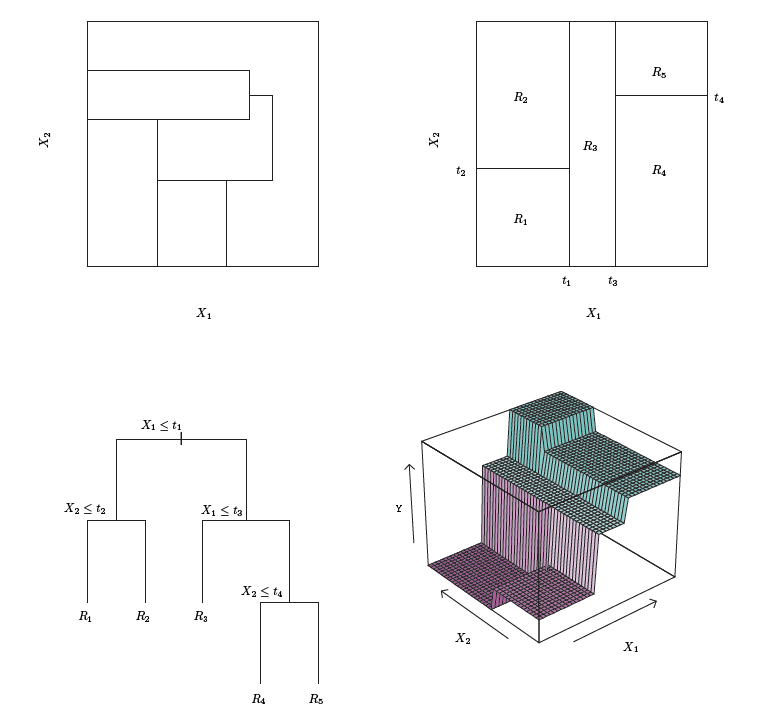
\includegraphics[height = 0.7\textwidth, width = \textwidth]{cart.png}
    \caption{A visualization of recursive binary splitting and tree growth. Figure from ISLR \citep{ISLR}}
    \label{cart}
\end{figure}


\subsection{Tree Prediction}
After growing a tree based on the training samples, we assign labels to the terminal nodes based on the most occurring classes of the observations in the terminal nodes. The final prediction of a new observation is decided by the assigned label of the terminal node the observation falls into. 

There are many great things about using decision trees in classification tasks such as easy interpretability and computation efficiency. However, trees are often non-robust and have large variance from sample to sample. In the next section, we will introduce random forests, a much more powerful predictive model that use trees as building blocks.

\section{Random Forests}

\subsection{Bootstrapping and Bagging}
Bootstrapping is widely used in statistics to approximate the unknown sampling distribution of a statistic. In the context of decision trees, the bootstrap can be particularly useful to improve the predictions themselves. The procedure of bootstrap is: take repeated samples which are the same size as the data with replacement. The underlying assumption is the original data are an accurate representation of the population and the bootstrap procedure allows us to emulate the process of obtaining new sample sets from the population. Through constructing bootstrap samples and averaging or majority vote on the predictions built on each sample, we can greatly reduce the variability of our predictions from different training samples. This technique is called bagging.

\begin{figure}[h]
\centering
\resizebox{1\textwidth}{!}{\begin{tabular}{cc}
  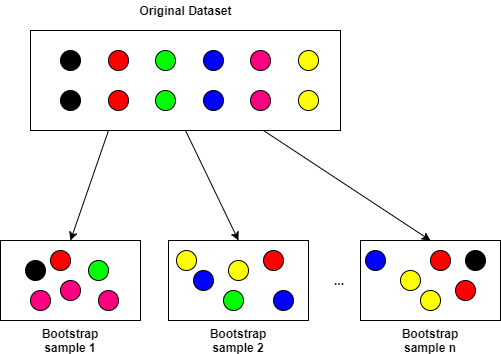
\includegraphics[width=\textwidth,height = 0.8\textwidth]{bootstrap_demo.png} &  \hspace{2mm} 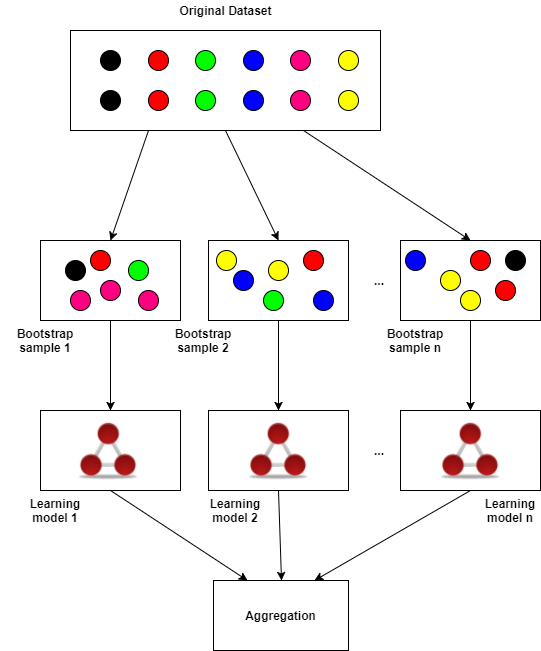
\includegraphics[width=\textwidth,height = \textwidth]{bagging-demo.png} \\
(a) Bootstrapping demo & (b) Bagging demo \\[8pt]
\end{tabular}}
\label{cohabitants-example-1}
\caption{An illustration of bootstrapping and bagging. This figures come from this \href{https://towardsdatascience.com/decision-trees-and-random-forests-for-classification-and-regression-pt-2-2b1fcd03e342}{tutorial on towardsdatascience.com}}. 
\end{figure}

\section {Constructing Random Forests}
The procedure of constructing a random forest follows from bagging. The only difference is, instead of looking through the entire predictor space, for each tree at each split, we only evaluate a randomly chosen subset of predictors to evaluate the splitting criteria. The procedure for random forest prediction is as follow:
\begin{enumerate}
    \item Bootstrap $B$ samples from the data $z_1,...z_n$.
    \item Grow classification trees $T_1, T_2,... T_B$ where $T_b$ is constructed on the $b$th bootstrap sample with $m$ randomly chosen predictors ($0<m<p$) considered at each split. 
    \item For a new observation, make predictions using each of the $B$ trees. The final prediction is the majority class of all $B$ predictions from $B$ trees.
\end{enumerate}

Since at each split only a random subset of the predictors are considered, the bagged trees will not be dominated by a single strong predictor. In such random forests are able to generate de-correlated trees, making the aggregated prediction less variable and more robust.  

\subsection{Out-of-Bag Estimation}
Each bootstrap sample is sampled with replacement from the original data, thus some observations from the original data might appear in the bootstrap sample while some might not. This property enables us to directly estimate random forests' predictive performance on new data. We will lay out the following definitions.

\begin{definition}
\label{oob-def}
Let $\varphi$ be a random forest with $B$ trees $T_1,...,T_B$. For the $b$th decision tree $T_b$, a training observation $z_i$ is \textbf{out-of-bag} if $z_i$ is not in the $b$th bootstrap sample.
\end{definition}

\begin{proposition}
\label{one-third}
On average, each bagged tree makes use of around 2/3 of the training observations. 
\end{proposition}

The proof to Proposition \ref{one-third} is fairly straightforward. $Pr(z_i$ not in a bootstrap sample) $= (1-\frac{1}{n})^n $. As $n \to \infty$, the probability converges to $\frac{1}{e} \approx \frac{1}{3}$. Therefore for each bagged tree, around 1/3 of the training data are out-of-bag.

\begin{definition}
\label{oob-prediction}
The out-of-bag prediction of a training observation $z_i$ is the majority vote over all predictions of $z_i$ by trees where $z_i$ is out-of-bag. Each training observation yields around $B/3$ such predictions toward the final out-of-bag prediction.
\end{definition}

We can use the out-of-bag prediction accuracy for all training data to estimate the predictive performance of the model on new observations since the out-of-bag prediction of each training sample is yielded only on trees that were not used to fit the sample. We will revisit out-of-bag prediction error estimation in the next chapter in our discussion of prediction confidence. We will also use the out-of-bag concept to construct local confidence in Chapter 5. 
\end{chapter}


%%%%%%%%%%%%% CHAPTER 4
%%%%%%%%%%%%%%%%% PREDICTION CONFIDENCE  %%%%%%%%%%
%%%%%%%%%%%%

\begin{chapter}{Prediction Confidence in Machine Learning Models}
In  classification tasks, in addition to the actual predictions, we are also interested in knowing how confident the model is in making the individual predictions. In other words, how likely is the model to be correct in predicting a new observation? Having an estimate of prediction confidence is particularly crucial in many real-world situations where classification results drive high-stake decision-making. 

This chapter will discuss existing metrics that are commonly used in the machine learning community to estimate prediction confidence and introduce the motivation behind our novel proposed method.


\section{Overall Training Accuracy}
The most common approach to quantify the learning model's predictive ability is to look at the training accuracy.

\begin{definition}
Let $z_1,...z_n$ be the set of training data. Let $y_1,...y_n$ be their true labels, and $\hat{y_1},...\hat{y_n}$ be the predicted labels. The training accuracy of the model is
\begin{equation}
\label{acc_train}
    Acc_{training}=\frac{\sum_{i=1}^n \mathbb{I}(\hat{y_i}=y_i)}{n}
\end{equation}
\end{definition}

However, assessing a model's prediction capacity on future data based on the data used to fit the model is problematic. Since the model is tuned to fit the training data closely, its prediction accuracy of new data will be overestimated by the training accuracy. 


\section{Test Accuracy}
Since we are interested in the model's performance on unseen data, a better idea for assessing accuracy is to create a test data set independent of model fitting. If we randomly sub-sample a part of our data and make predictions after the model is fitted, the prediction accuracy on the test data set will approximate that on future new observations, assuming that the test data is representative of the population. 

\begin{definition}
Let $z_1*,...z_m*$ be the set of test data. Let $y_1*,...y_m*$ be their true labels, and $\hat{y_1*},...\hat{y_m*}$ be the predicted labels. The test accuracy of the model is
\begin{equation}
\label{acc_test}
    Acc_{test}=\frac{\sum_{i=1}^m \mathbb{I}(\hat{y_i*}=y_i*)}{m}
\end{equation}
\end{definition}


% \begin{figure}[h]
%     \centering
%     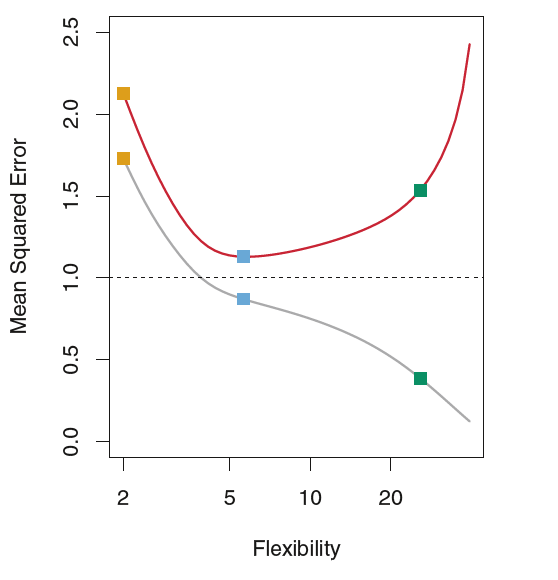
\includegraphics{train-test-mse.png}
%     \caption{Training MSE (grey curve), test MSE (red
% curve), and minimum possible test MSE over all methods (dashed line). Squares represent the training and test MSEs for the three fits (linear regression, orange, and two smoothing splines, blue and green) shown in the left-hand panel. Figure cited from ISLR (\cite{ISLR})}
%     \label{train_test}
% \end{figure}\\

% The training error decreases monotonically as flexibility increases. However, the test error does not always decrease with the training error: after hitting the bottom, the test error increases as training error keeps decreasing. When a model has a much larger test error than training, it is overfitting the data. For the scope of this thesis, we will not talk about methods of fitting the best model. Instead, we assume that the model is fitted with optimal bias-variance trade-off. That being said, we can observe that training error is always lower than test error. 

However, splitting data into train and test will result in fewer data for the training set, making the training set less representative. This problem will become especially prominent with a small sample size. 
%\section{Cross-Validation Accuracy}

\section{Out-of-bag Training Accuracy}
In random forests, instead of a train-test split we can also assess prediction accuracy on new data with training observations only using out-of-bag predictions. Since each bootstrap sample uses approximately 2/3 of the data, and each training observation is not included in the building of around 1/3 trees, we can conveniently use the training set to assess our model's prediction accuracy on new data. We define this metric out-of-bag training accuracy.

Recall the definition of out-of-bag predictions from \ref{oob-prediction}. 

\begin{definition}
Let $\hat{y}_{-1},...\hat{y}_{-n}$ be the out-of-bag predictions for training observations $z_1,...z_n$. The \textbf{out-of-bag training accuracy} is 
\begin{equation}
\label{acc_oob}
   Acc_{oob}=\frac{\sum_{i=1}^n \mathbb{1}(\hat{y}_{-i}=y_i)}{n}
\end{equation}
\end{definition}

A shared problem with the confidence metrics we have discussed so far is none of them directly considers the prediction confidence of individual new observations. The underlying concept behind training, test and out-of-bag accuracy is we can approximate the prediction accuracy of a set of future data using accuracy of a set of known data. However, the model's ability to predict observations in different feature spaces could be immensely different.

We will illustrate our point with an example. Suppose our data consists of two clusters, with one mixed and one homogeneous classes. Our learning models will perform poorly on the mixed group, resulting in around $50\%$ accuracy. However, the model will predict almost perfectly on the homogeneous cluster. Therefore, although the overall accuracy is $75\%$, that number itself is not representative of the true prediction accuracy of the individual samples in either of the two different clusters. 

\begin{figure}[h]
    \centering
    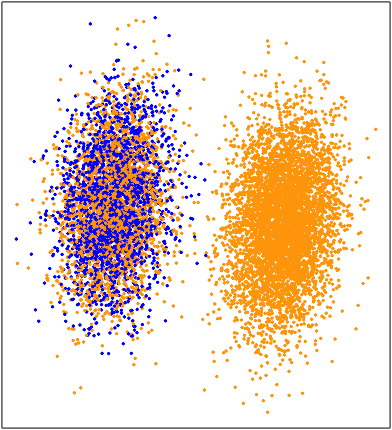
\includegraphics[scale=0.26]{cluster1.png}
    \caption{An example of when an overall accuracy metric falls short}
    \label{local_confidence_demo}
\end{figure}

Therefore, we are motivated to find a prediction confidence metric of individual new data, drawing parallels to the idea of constructing prediction intervals in linear regression. 

Interestingly, the aggregate nature of random forests allows us to obtain a confidence estimation of individual observations. 

\section{Class Probabilities}
Since random forests are an ensemble learner, a common approach to estimate the prediction confidence of a new observation is to use the proportion of trees that voted the final prediction class. This proportion is also interpreted as the the probability of the prediction being in the predicted class.
\begin{definition}
Let $\varphi$ be a Random Forests with $B$ trees $T_1,...,T_B$ and our data has a categorical response of $K$ levels. For a new observation $z_h$, if the predicted response is $k \in \{1,....,K\}$, then the probability that $z_h$ has a response of $k$ is
\begin{equation}
\label{prob}
    p_h=\frac{1}{B}\sum_{b=1}^B \mathbb{1} (\hat{y}_b=k)
\end{equation}
where $\hat{y}_b$ is the predicted response from the $b$th tree.
We also refer to this probability as class probability.
\end{definition}

The class probability  $p_h$ is $1$ if the predicted responses by all trees are $k$, meaning that the model is very confident in its prediction of $z_h$. By the majority vote rule and pigeonhole principle, $p_h$ must not be smaller than $\frac{1}{k}$.  The smaller $p_h$ is, the less confident we are about the prediction.

However, in calculating class probability, we are considering all trees including those built on bootstrap samples that are irrelevant or distracting to the new observation to be predicted. Having predictions from those trees could add noise to our estimate of prediction confidence. 

To conclude, all the metrics examined in this chapter use a global approach to estimate the prediction confidence of a new observation. That is, the metrics indiscriminately use the model's ability to predict all observations to estimate the confidence of one new observation. We argue that a global metric is not necessary, and if we only look at observations locally, we can have a direct improvement on our confidence metric.  
\end{chapter}


% \section{Discussion}
% Most of the confidence metrics discussed in this chapter give an overall accuracy, the proportion of a set of data that is predicted correctly. However, drawing a parallel with Chapter 2 on confidence vs prediction interval, we also want a metric that measures the prediction confidence of individual observations. 

% We will illustrate the motivation with an example. Suppose our data is consisted of two clusters, with one mixed and one homogeneous. Our learning models will perform poorly on the mixed group, resulting in around $50\%$ accuracy. However, the model will predict almost perfectly on the homogeneous cluster. Therefore, although the overall accuracy is $75\%$, it is not representative of the true prediction accuracy of individual points. 

% \begin{figure}[h]
%     \centering
%     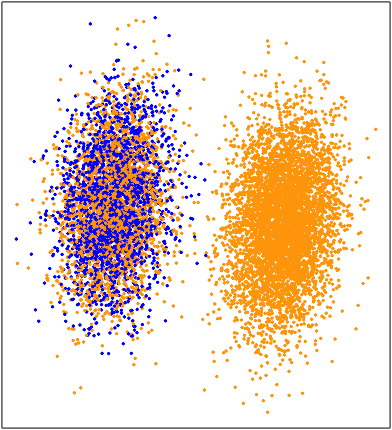
\includegraphics[scale=0.26]{cluster1.png}
%     \caption{An example of when an overall accuracy metric falls short}
%     \label{local_confidence_demo}
% \end{figure}


%%%%%%%%%%%%%%%%%%% LOCAL PREDICTION CONFIDENCE 
\begin{chapter}{Local Prediction Confidence}
\indent Following the previous chapter, we propose a local prediction confidence metric for individual observations. We define local prediction confidence in a frequentist fashion, as the percentage of the random forests models, among repeated samples, that predict the response class correctly given a specific feature space. We approximate the local prediction confidence of a new observation with the model's prediction accuracy on other training observations, weighted by the similarity between the training observations and the new observation . This locally weighted approach has been adopted in optimizing forests building in the context of generalized random forests \citep{grf}. It is theoretically reasonable to use the same approach to estimate prediction confidence to filter noises irrelevant to individual observations. 

\section{Define Local Confidence}
In \cite{JMLR}, a prediction confidence interval is constructed with locally weighted error. We will adopt a similar idea in our construction of a local confidence metric.

\begin{definition}
A training observation is an \textbf{out-of-bag cohabitant} with the new observation in a tree if
\begin{itemize}
    \item the training observation is out-of-bag in this tree
    \item the training observation ends up in the same terminal node
with the new observation
\end{itemize}
\end{definition}

The oob-cohabitance frequency can be used as a relevance measure of a training observation to the prediction of the new observation \citep{grf}. We believe that the more frequent the training observation out-of-bag-cohabits with the new observation, the more likely they come from the same class label. Therefore, more weights should be given to random forests' predictive accuracy on the more relevant training observations. 

Now let's define our local confidence score.

\begin{definition}
Let $z_1,...z_n$ be the training observations. Let $z_h$ be the new observation we want to predict. Let $w_i$ be the number of times a training observation $z_i$ out-of-bag-cohabits with $z_h$. 

Let $\hat{y}_{-i}$ be the out of bag prediction for $z_i$. Then
     \begin{equation}
     \label{local}
         local\_confidence(z_h) = \frac{1}{\sum w_i}\sum_{i=1}^{n} w_i \mathbb{I}(\hat{y}_{(-i)}=y_i)
     \end{equation}  
\end{definition}


The intuition behind our construction is that we will estimate the prediction confidence of a new observation with the oob prediction accuracy of local training samples. If a training observation, when it is out-of-bag, never falls in the same terminal node with the new observation, then its out-of-bag prediction accuracy will not be considered in the local confidence score. In this way, our metric is able to exclude the predictive performance of training observations that come from a different class. On the other hand, the more frequent a training observation out-of-bag cohabits with the new observation, the more likely they come from the same class.

A local confidence metric has an advantage over a global metric when data exhibits significant heterogeneity, or the model's predictive power varies greatly in different feature space. The following chapter will create multiple scenarios and use simulations to compare different metrics.
\end{chapter}




%%%%%%%%%%%%%%%%%%%%%%%%%%%%%%% EVALUATION %%%%%%%%%%%%%%%%%%%%%%%%%%%%
\begin{chapter}{Evaluation}

This chapter will introduce simulation methods to compare different prediction confidence metrics. We will create scenarios where some metrics outperforms the others and the other way around.

\section{Approximate True Prediction Confidence}
The first step in comparing metrics is creating a benchmark. In other words, how can we know the ``true" prediction confidence of a new observation? 

We begin with simulating a population with designed characteristics, and repeatedly drawing smaller sub-samples to make predictions on the new observation. The approximated ``true" prediction confidence will be the proportion of correct predictions among the repeated samples. 

In real-life research, scientists most likely get only one data sample. A confidence metric is obtained from that one particular sample, and there is no way to verify if it is biased or not. However, through simulating a population and repeatedly taking sub-samples, our method is able to assess the random forests' ability to predict the new observation based on different training samples. Ideally, if we have the ability to collect all possible samples from the population, then the prediction accuracy of the models trained by all samples represents the random forests' confidence of predicting the new observation. This construction is extremely similar to the definition of confidence intervals in linear regression.

We define the proportion of correct predictions among all possible training data the ``true" prediction confidence, and claim that the result generated by our algorithm well approximates the true confidence. \\\\

\newline
\hline
\vspace{0.05in}
\textbf{Algorithm 2} Simulate True Prediction Confidence
\vspace{0.05in}
\hline
\begin{algorithm}
\label{avg_confidence}
\label{split}
\begin{algorithmc}
\Procedure{trueConfidence} {A population of size N, sample size n, new observation $z_h$}
 \State Simulate a population of size N and initialize count = 0
 \For{j in 1,2,...num$\_$iterations}
 \State Take a sample of size n from the population without replacement.
 \State Train a random forest on the sample.
 \State Use the random forest to make a prediction on $z_h$. count + 1 if the prediction is correct.
 \EndFor
 \State Return $true\_confidednce$ = count/num$\_$iterations
 
\EndProcedure
\newline
\end{algorithmc}
\end{algorithm}

\vspace{2mm}
We used Ranger \citep{ranger}, an R package for fast implementation of Random Forests, to train the models. All the random forests are tuned with default values specified by Ranger, so that the model parameters are controlled across all training samples. 

We empirically evaluated the number of iterations needed for the algorithm to converge by comparing the differences of absolute prediction confidence scores between the current iteration and previous iteration. We simulated a population with two Gaussian clusters, 20 features, N = 10,000 and n = 1000, and a test set of size 500. 

\begin{table}[h]
\centering
\label{convergencetable}
\begin{tabular}{|l|l|l|l|l|}
\hline
n\_features \textbackslash{}num\_iteration & 50     & 100    & 500    & 1000   \\
\hline
10                                         & 0.05   & 0.0269 & 0.0178 & 0.008  \\
20                                         & 0.0689 & 0.0332 & 0.0215 & 0.0111 \\
50                                         & 0.0864 & 0.0384 & 0.0279 & 0.0129\\
\hline

\end{tabular}

\caption{Average absolute differences of confidence scores compared to the previous iteration. 50 iterations is compared to 10 iterations.}
\end{table}

From Table \ref{convergencetable}, we can observe that starting from 100 iterations and above, the scores returned by the algorithm differ much less than scores from the previous iterations. Therefore, we use 100 iterations to achieve fast and accurate implementation of true confidence approximation. 

\section{Simulations}
In this section, we will create multiple data scenarios to test the metrics discussed in Chapter 4 and 5. The goal is to give concrete evidence of which confidence metrics most accurately describe population structures. We will also discuss the scenarios when local confidence does not have a substantial advantage. 

We used Python's sklearn package to simulate datasets for classification \citep{sklearn}. Each population consists of clusters of points normally distributed (std=1) about vertices of a hyper-cube or polytope whose dimension and size are based on the number of informative features and the extent of class separation. In this thesis, we only focus on binary classification. 

There are multiple parameters that we can control:
\begin{itemize}
    \item n$\_$features: the number of features.
    \item n$\_$informative: the number of informative features.
    \item n$\_$redundant: the number of redundant features.
    \item n$\_$repeated: the number of repeated features, which are randomly generated as a linear combination of informative features.
    \item n$\_$classes and n$\_$clusters per class: the number of classes and number of clusters per class. A class can have multiple clusters each with a different spread in feature space. In this thesis, n$\_$classes = 2.
    
    \item flip$\_$y: the proportion of class labels that are randomly switched. A large value introduces more noise.
    \item class$\_$sep: the factor multiplying the hyper-cube size. A larger values spreads out the clusters and make the classification task easier.
    \item hypercube: true if the clusters are put on the vertices of a hypercube or put on the vertices of a random polytope.
\end{itemize}


% \begin{table}[h]
%     \resizebox{\textwidth}{!}{\begin{tabular}{|l|l|}
%     \hline
%     parameters & description \\
%     \hline
%      n$\_$informative & the number of informative features\\
%      \hline
%      n$\_$redundant & the number of redundant features \\
%      \hline
%      n$\_$repeated& the number of repeated features, which are randomly generated\\  & as a linear combination of informative features \\
%      \hline
%      n$\_$classes and n$\_$clusters per class& the number of classes and number of clusters per class \\
%      \hline
%      weights& the proportion of samples assigned to each class\\
%      \hline
%      flip$\_$y& the proportion of class labels that are randomly switched.\\  & A large value introduced more noise\\
%      \hline
%      class$\_$sep& the factor multiplying the hyper-cube size.\\ & Larger values spread out the clusters and make the classification task easier\\
%      \hline
%      hypercube& true if the clusters are put on the vertices of a hypercube \\ & or put on the vertices of a random polytope\\
%      \hline
%     \end{tabular}}
%     \caption{Caption}
%     \label{tab:my_label}
% \end{table}


\hspace{1mm}

We designed populations using different combinations of the above parameters. They key questions to investigate are:
\begin{itemize}
    \item How good are the confidence metrics when the classes are homogeneous versus heterogeneous?
       \item How do confidence metrics change when data is high-dimensional?
    \item What happens with noisy or highly correlated features?
\end{itemize}

The simulation procedure consists of three parts: creating a population based on the question we want to investigate, approximating the true prediction confidence, and calculating prediction confidence on a random training sample from the population. \\

\hline
\vspace{0.05in}
\textbf{Algorithm 3} Create a Population
\vspace{0.05in}
\hline
\begin{algorithm}
\label{make_population}
\label{split}
\begin{algorithmc}
\Procedure{makePopulation} {population size $N$, n$\_$features, n$\_$informative, n$\_$redundant and other data parameters to be evaluated, heterogeneity parameter $p_1$,...,$p_{n\_cluster}$}
 \State Use sklearn.datasets.make$\_$classification to generate a dataset with the set of parameters we specify in each data scenario. 
 \State Within each cluster $i$, randomly flip $p_i$ of the observations to the other class.
\EndProcedure
\newline
\end{algorithmc}
\end{algorithm}

\newline
\hline
\vspace{0.05in}
\textbf{Algorithm 4} Simulation Procedure
\vspace{0.05in}
\hline
\begin{algorithm}
\label{simulation}
\label{split}
\begin{algorithmc}
\Procedure{simulation} {The set of parameters for population generation,training sample size $n$, test sample size $m$}
 \State run $makePopulation$ to create a population.
 \State Take $m$ random observations from the population as the test set. We treat this test set as "new" data.
 \State Take $n$ random observations from the population as a real-life training sample.
 \State Use the rest of the population to find true prediction confidence of the new data with $trueConfidence$.
 \State Use the training sample to calculate the confidence metrics and compare them with the true confidence. 
 \State Return $Acc_{oob}$, $Acc_{test}$, $local\_confidence(test)$, $true\_confidence(test)$ 
 
\EndProcedure
\newline
\end{algorithmc}
\end{algorithm}


\section{Simulation Results}
\begin{example}
\label{example1}
We begin with a simple example to visually understand the confidence machinery. Simulate a population of 10,000 observations, two classes with one cluster per class, and two informative features. Randomly switch the class label of half of the observations to the other class in the yellow cluster and the blue cluster remains unchanged. 

 simulation($N=10,000$, $n=1000$, $m=500$, n$\_$clusters$\_$per$\_$class $= 1$, and n$\_$features$=$n$\_$informative$=2$, p$\_$yellow$=0.5$, p$\_$blue$=0$.

\begin{figure}[h]
    \centering
    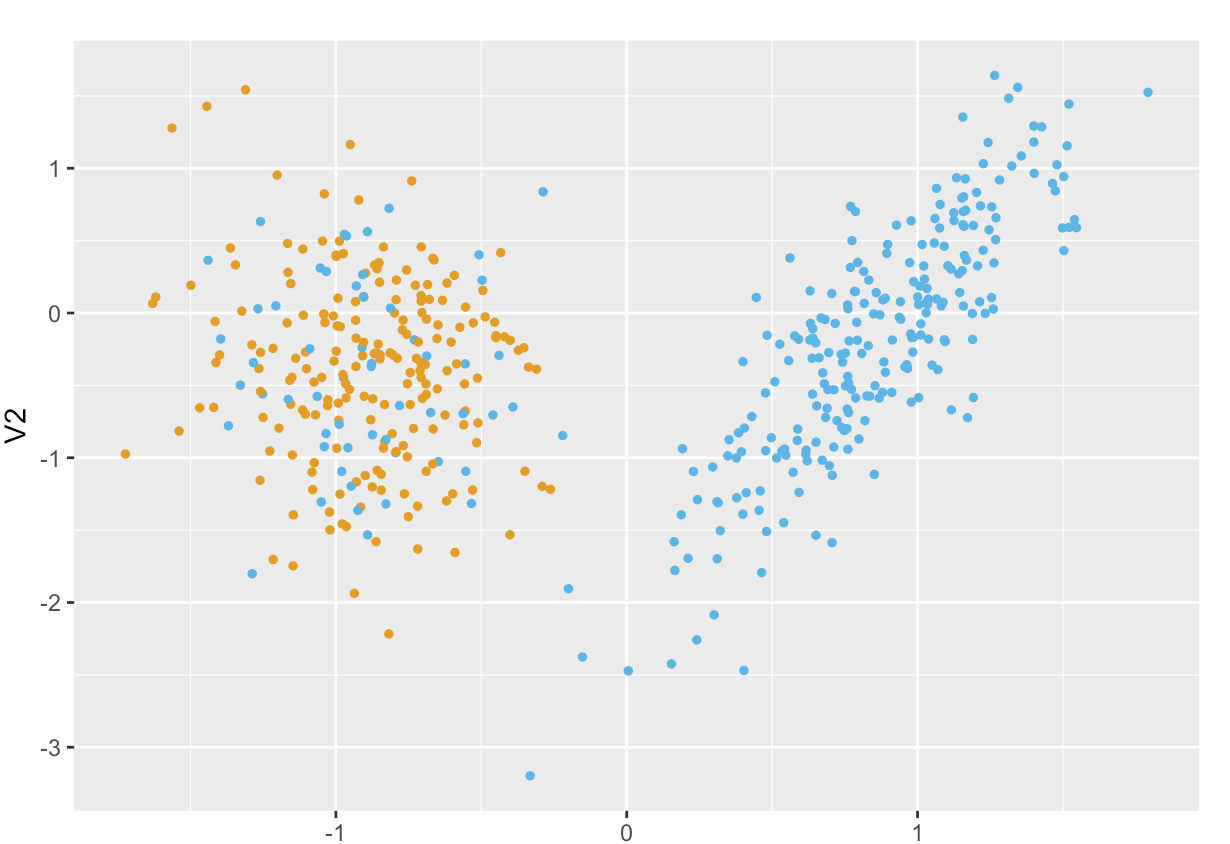
\includegraphics[scale=0.5]{example1.png}
    \caption{Visualization of the population in Example \ref{example1}}
    \label{trivial example}
\end{figure}
\end{example}

The random forests are built with n$\_$tree$ = 50$. We pruned the trees by specifying the minimum node size. The most optimal node size was selected by oob-error. In this example, the minimum node size is $20$. We can observe that the random forests can perfectly predict the homogeneous cluster but not the heterogeneous one because both yellow and blue classes share the same feature space in this cluster.

We take three observations from the test set for comparisons. One blue point from the heterogeneous cluster on the left, one blue from the homogeneous cluster on the right, and one yellow point.  The three test observations and their cohabitants are in the following figure. 

\begin{figure}[h]
\centering
\resizebox{1\textwidth}{!}{\begin{tabular}{cc}
  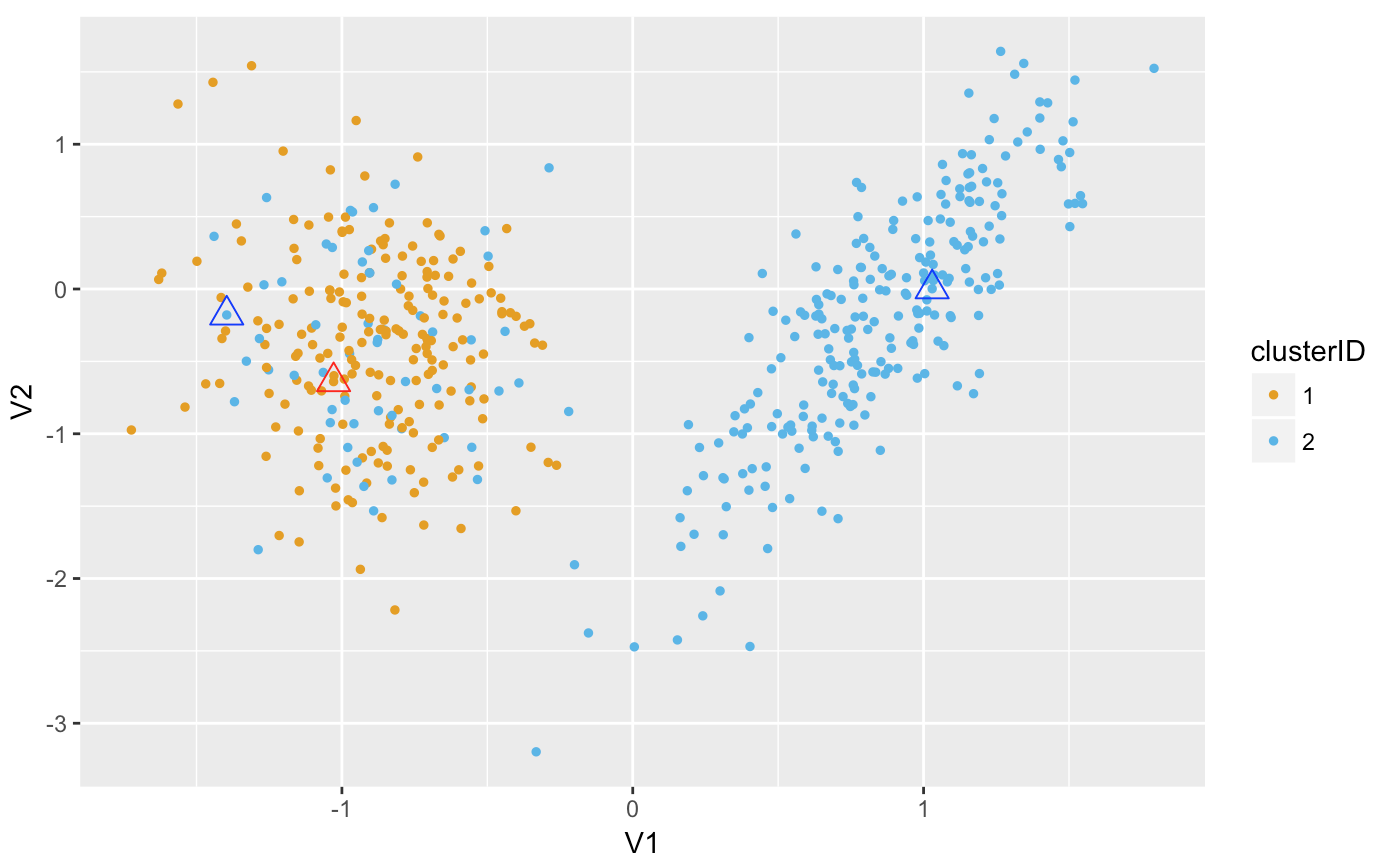
\includegraphics[width=\textwidth,height = 0.8\textwidth]{example1_1.png} &   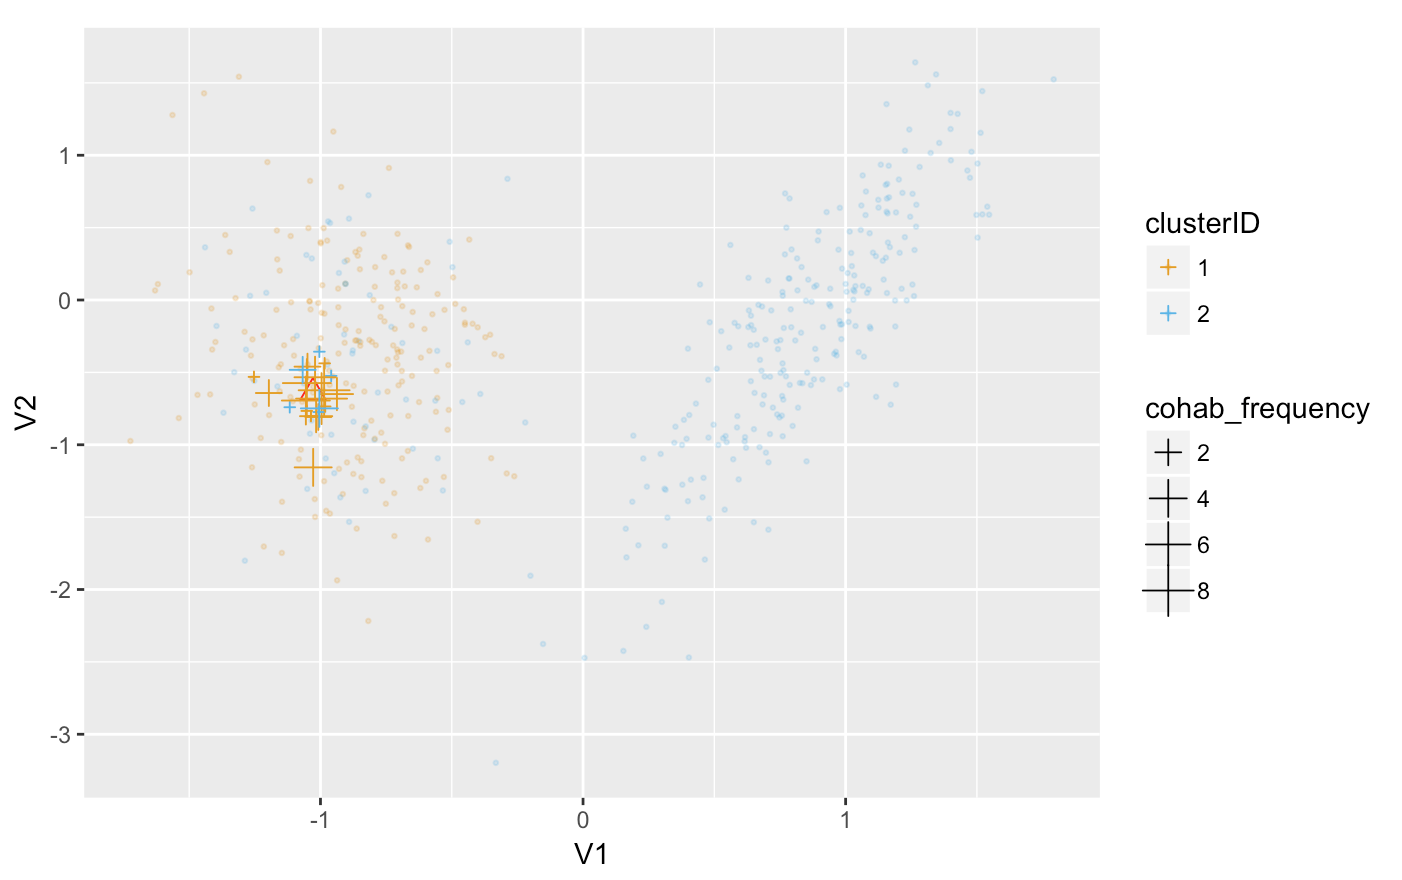
\includegraphics[width=1.1\textwidth,height = 0.81\textwidth]{example1_2.png} \\
(a) The three benchmark test observations highlighted in triangles & (b) Cohabitants of the yellow observation \\[6pt]
 \hspace{3mm}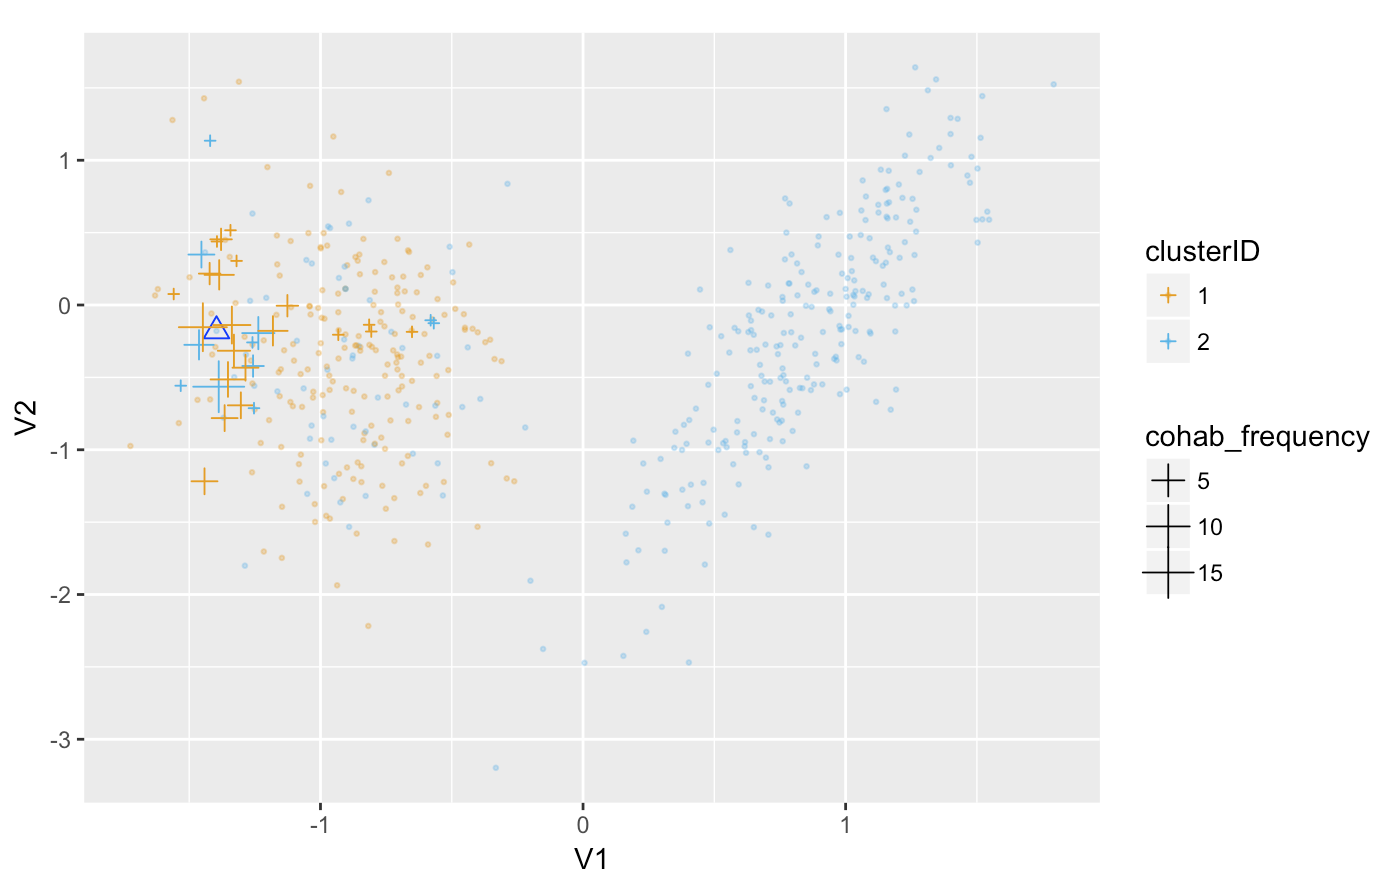
\includegraphics[width=1.1\textwidth,height = 0.8\textwidth]{example1_3.png} &   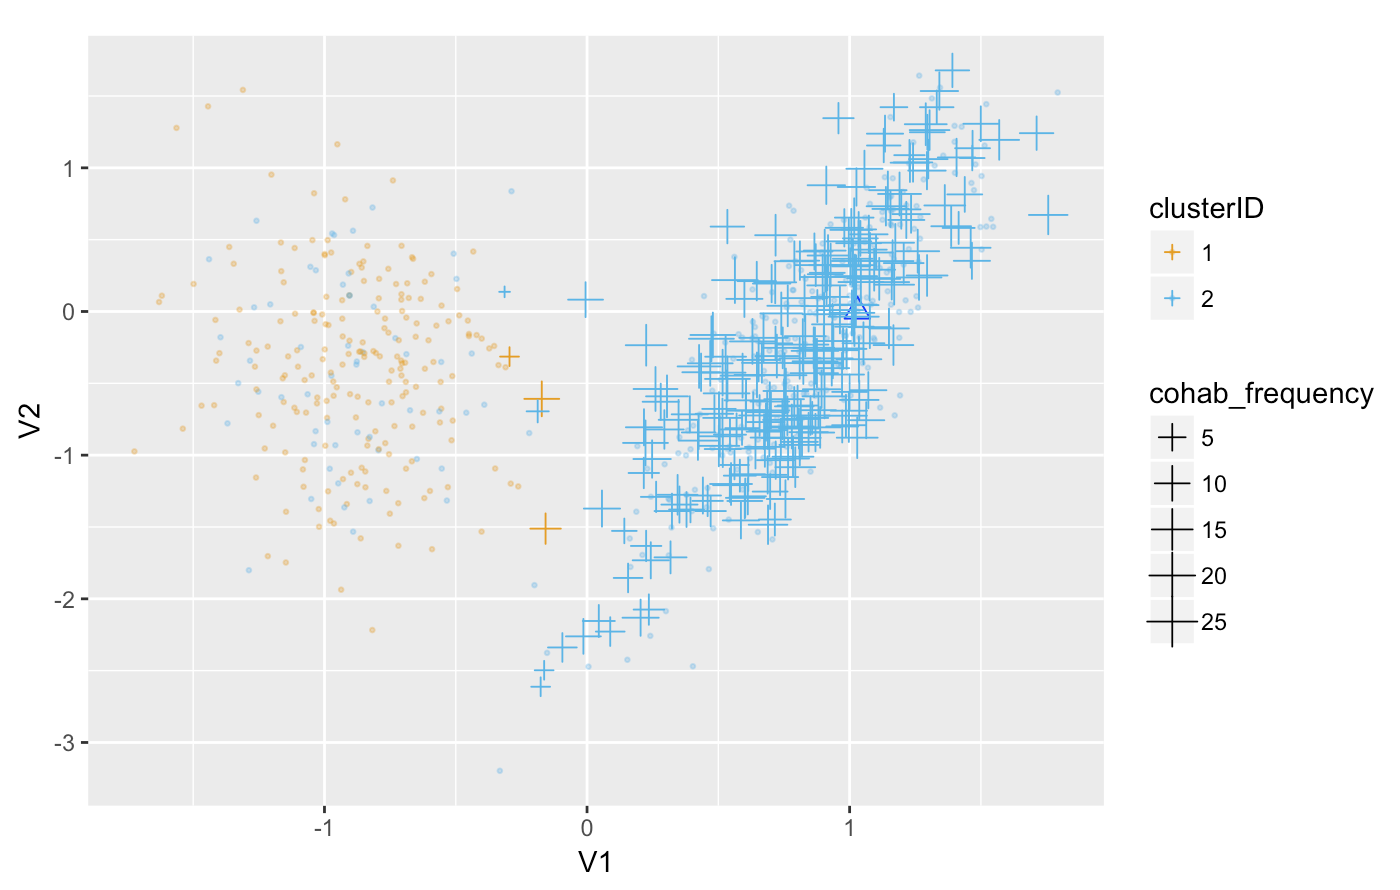
\includegraphics[width=1.1\textwidth,height = 0.8\textwidth]{example1_4.png} \\
(c) Cohabitants of the blue observation from the left cluster & (d) Cohabitants of the blue observation from the right cluster \\[6pt]
\end{tabular}}
\label{cohabitants-example-1}
\caption{A visualization of the cohabitants. All cohabitants are of the ``+" shape. The size are determined by the frequency of the cohabitance. A random half of the cohabitants are plotted to avoid over-crowding the plots.}
\end{figure}
\newpage
The confidence metrics of the three observations are summarized in Table \ref{table1} and \ref{confusion matrix}. 

\begin{table}[h]
    \centering
    \begin{tabular}{|l|l|l|l|}
    \hline
         & blue from heterogeneous & blue from homogeneous  & yellow \\
         \hline
         $Acc_{oob}$ (\ref{acc_oob}) & 0.842 & 0.842 & 0.842 \\
         \hline
         $Acc_{test}$ (\ref{acc_test})  & 0.856 & 0.856 & 0.856  \\
         \hline
         $p_h$ (\ref{prob})   & 1 & 0.56 & 0.74  \\
         \hline
         $local\_confidence$ (\ref{avg_confidence}) & 0.727 & 0.996 & 0.833  \\
         \hline
         $true\_confidence$ (\ref{local}) & 0.08 & 1 & 0.85   \\
         \hline 
         
    \end{tabular}
    \caption{A summary of confidence metrics on Example \ref{example1}}
    \label{table1}
\end{table}

\begin{table}[h]
    \centering
    
     \begin{tabular}{|l|l|l|}
    \hline
         & Actual Yellow & Actual Blue \\
         \hline
         Predicted Yellow & 183 & 61 \\
         \hline
         Predicted Blue &11 &245 \\
         \hline
         Yellow Accuracy & 0.943 &-\ \\
         \hline
         Blue Accuracy & - & 0.801 \\
         \hline
         
    \end{tabular}
    \caption{Confusion matrix of test data}
    \label{confusion matrix}
\end{table}
The overall metrics, $Acc_{oob}$ and $Acc_{test}$ fail to differentiate between a blue point from the homogeneous cluster and a blue point from the heterogeneous cluster. Even though the overall accuracy on the entire test set is more than 80\%, the model performs badly on the heterogeneous cluster, which is not reflected in the overall metric's score. Even if we break down the overall accuracy by class, the test accuracy of the blue class is still inflated by the homogeneous cluster (by Table \ref{confusion matrix}), thus not accurately showing the model's predictive capacity on observations living in the heterogeneous space.

\begin{figure}[h]
\centering
\resizebox{.9\textwidth}{!}{
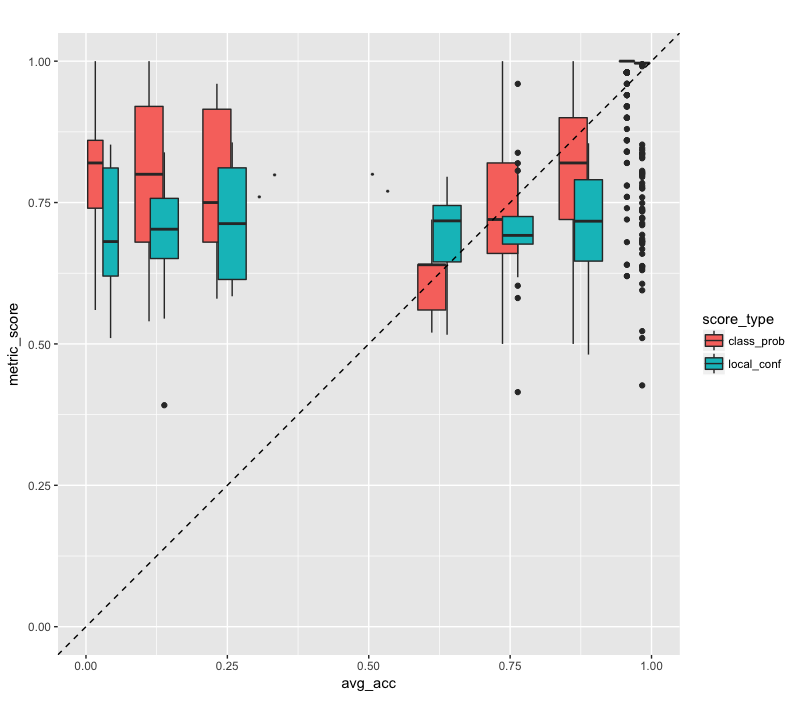
\includegraphics[width=1\textwidth,height = 0.8\textwidth]{example1_6.png} 
% \begin{tabular}{cc}
%   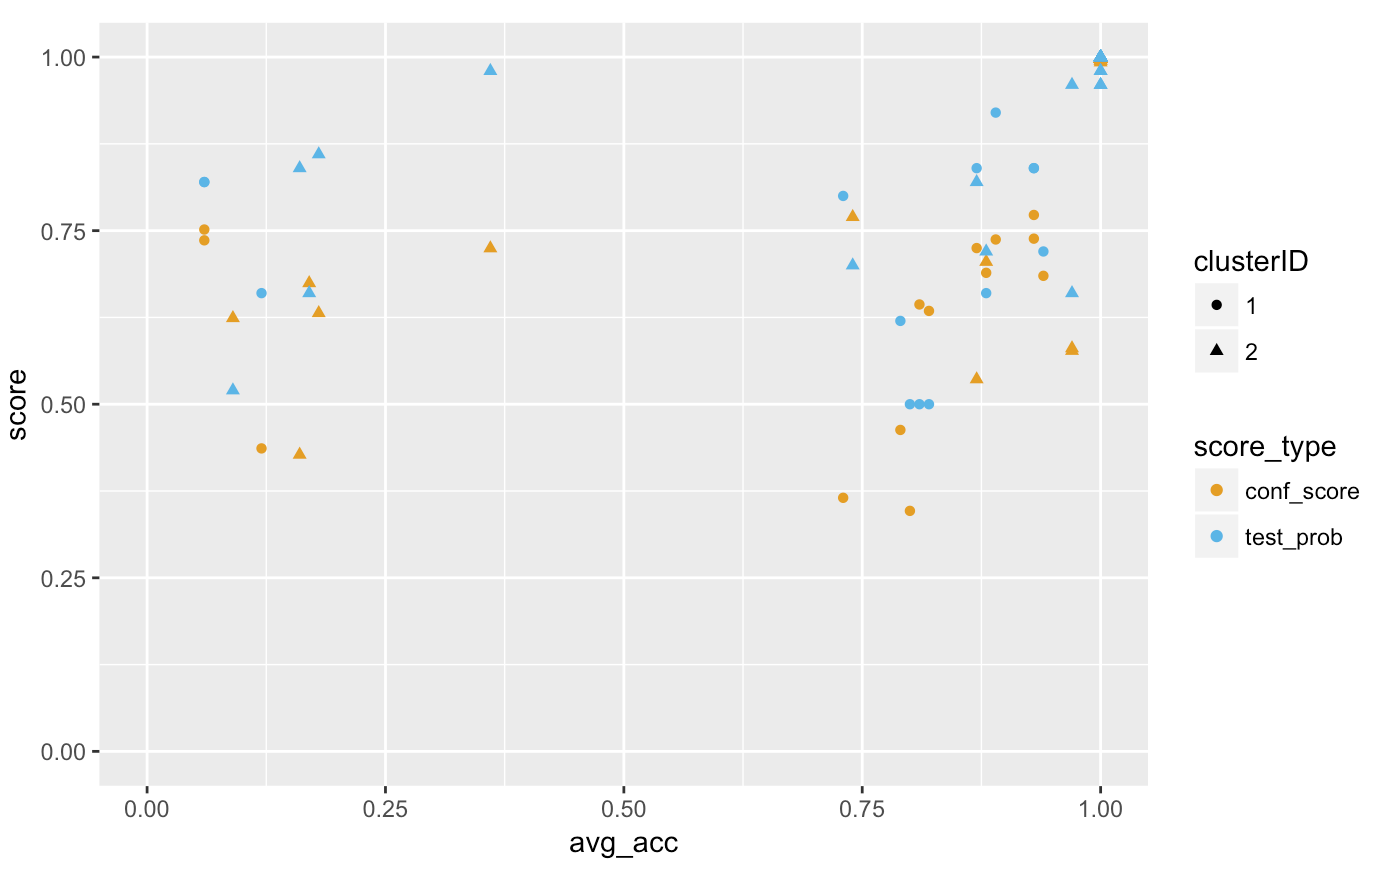
\includegraphics[width=\textwidth,height = 0.83\textwidth]{example1_5.png} &   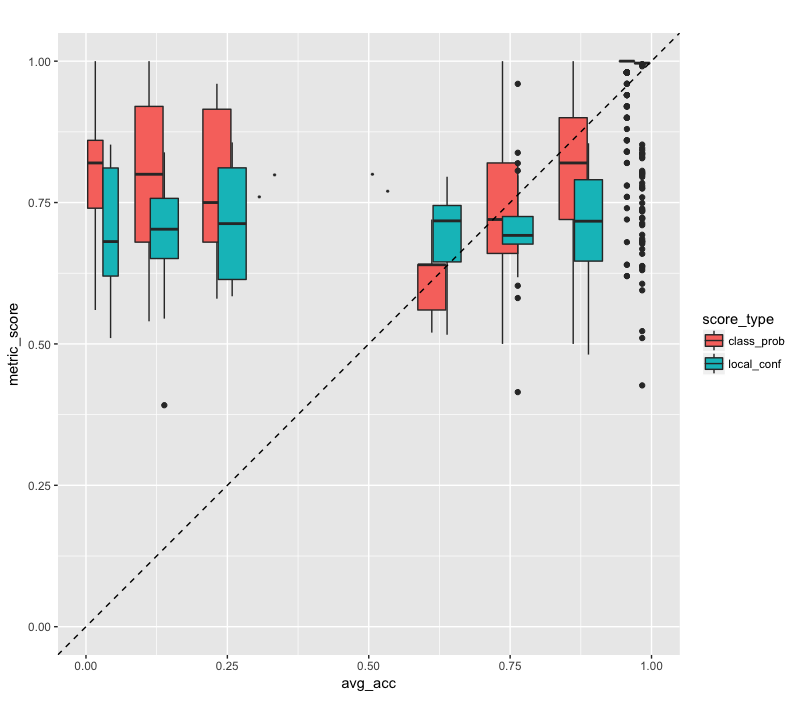
\includegraphics[width=1.1\textwidth,height = 0.81\textwidth]{example1_6.png} 
% \end{tabular}
}
\label{scores-example-1}
\caption{Comparisons between local confidence score and class probability on Example \ref{example1}. All test observations are plotted. The dashed line is the line of y=x, therefore the closer each test observation's metric is to the dashed line, the better the metric is.}
\end{figure}

To further compare local confidence and class probability, we plot confidence score versus class probability over the entire test set in Figure \ref{scores-example-1}. Between the class probability and the proposed local confidence score, it appears that local confidence is closer to the true prediction confidence especially in not perfectly confident predictions.  In Figure \ref{scores-example-1}, for observations with true confidence lower than $0.5$, the local confidence scores gives much lower estimates than class probability scores. For observations with true confidence greater than 0.5, both scores do fairly well. It is also worthy to note that local confidence score in general has less variance than class probability, making it a potentially better estimator. 


%This observation fits the random forests intuition. If we look closely at the composition of the yellow observation's cohabitants, we can find a mix of blue and yellow classes. By nature since the out-of-bag predictions for the heterogeneous cluster are correct almost half of the time, the local confidence score for both yellow and blue classes are around 0.6. However, for each test observation, if 60\% of the trees make the correct predictions, then the final result is correct. Despite false predictions, if the majority of trees vote towards one class, the class probability would still yield a large number. Therefore class probability is always higher for all three observations. 

%It is also true that local confidence is much smaller than the approximated true confidence in the yellow class case. Using the intuition we  just mentioned, we can argue that since more than 50\% of the trees voted towards the correct class, both class probability and true confidence scores are high. However, the proportion of trees is not much higher than 50\%, thus not making the prediction very ``confident". Therefore, the local confidence metric captures a nuance that neither approximated true confidence nor class probability has. In one way, local confidence score is more indicative of the heterogeneity in the feature space. 

Even though this is too small of an example to justify why local confidence metric is better in wider applications, we do gain a high level intuition of the local confidence machinery. We can also make the initial hypothesis that local confidence does offer a better alternative to overall out-of-bag accuracy to capture the heterogeneity of the feature space, and in some situations perform better than class probability. We will explore more cases and repeated large-scale simulations to further that hypothesis.

\begin{example}
\label{example2}
In this example, we seek to investigate the performance of the confidence metrics when the data is high-dimensional. The same basic set-up from the previous example is used with in an increased number of features to 50. The random forests have $n\_tree = 100$ and $min.node.size = 30$.

simulation($N=10,000$, $n=1000$, $m=500$, n$\_$clusters$\_$per$\_$class $= 1$, and n$\_$features$=$n$\_$informative$=50$, p$\_$yellow$=0.5$, p$\_$blue$=0$.
\end{example}

\begin{figure}[h]
\label{fig2}
\centering
\resizebox{.9\textwidth}{!}{
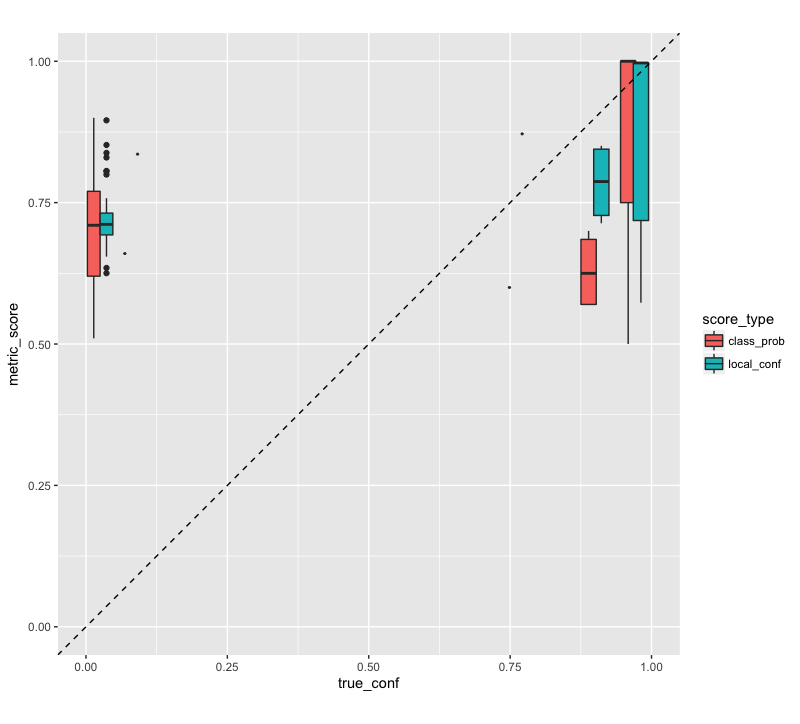
\includegraphics[width=1\textwidth,height = 0.8\textwidth]{example2_2.png} 
% \begin{tabular}{cc}
%   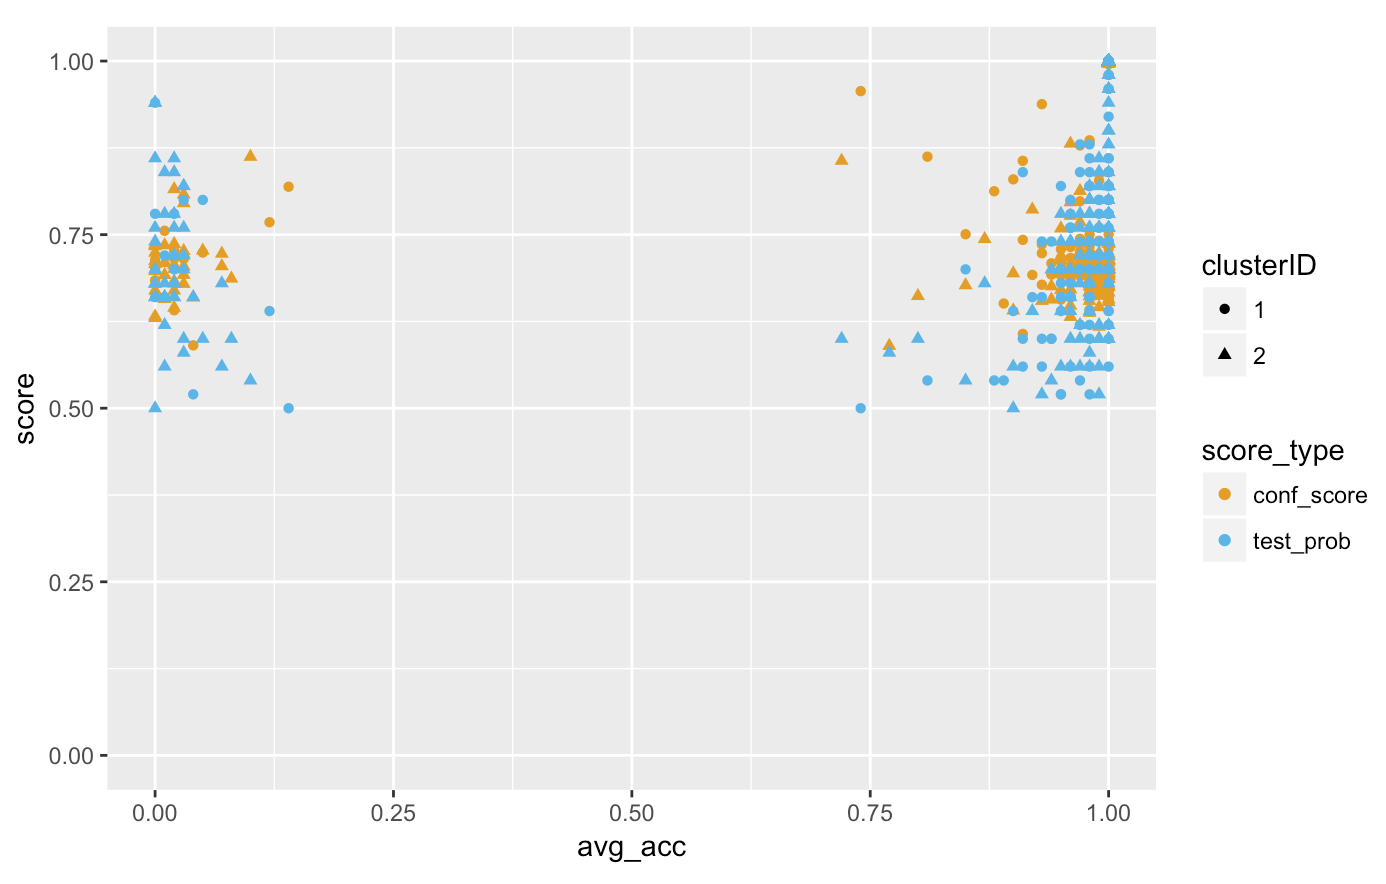
\includegraphics[width=\textwidth,height = 0.8\textwidth]{example2_1.png} &   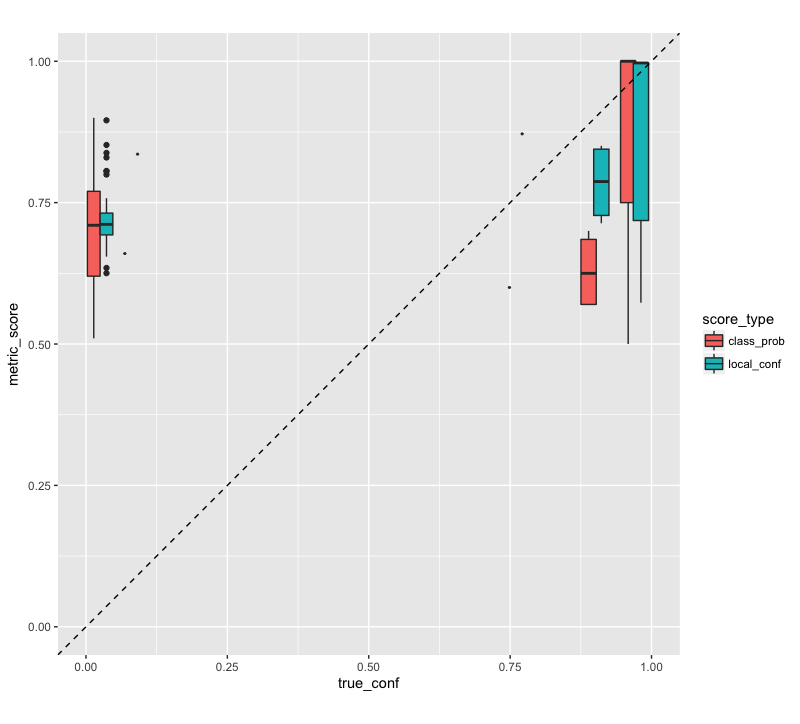
\includegraphics[width=1.1\textwidth,height = 0.8\textwidth]{example2_2.png} 
% \end{tabular}
}

\caption{Comparisons between local confidence score and class probability on Example \ref{example2}. All test observations are plotted.}
\end{figure}

The out-of-bag accuracy for all training data is 0.855 and test accuracy is 0.864. We see a slight improvement in overall accuracy because the high dimension enables the model to draw more separable boundaries. The local confidence score, class probability and true confidence are plotted in Figure 6.4. However, the result on high-dimensional data is not entirely consistent with the low-dimensional case since local confidence is not much better than the class probability. For a more rigorous argument, we will soon define metrics to quantify the differences between confidence metrics. 



\begin{example}
\label{example3}
With a high dimensional data we are now concerned with noisy or correlated features. We will begin with noisy feature only. With other parameters in the previous example controlled, we run simulations with 30 informative features and 20 noisy features.

simulation($N=10,000$, $n=1000$, $m=500$, n$\_$clusters$\_$per$\_$class $= 1$, and n$\_$features$=50$, n$\_$informative$=30$, n$\_$repeated $=20$, p$\_$yellow$=0.5$, p$\_$blue$=0$.
\end{example}

\begin{figure}[h]
\centering
\resizebox{.9\textwidth}{!}{
% \begin{tabular}{cc}
%   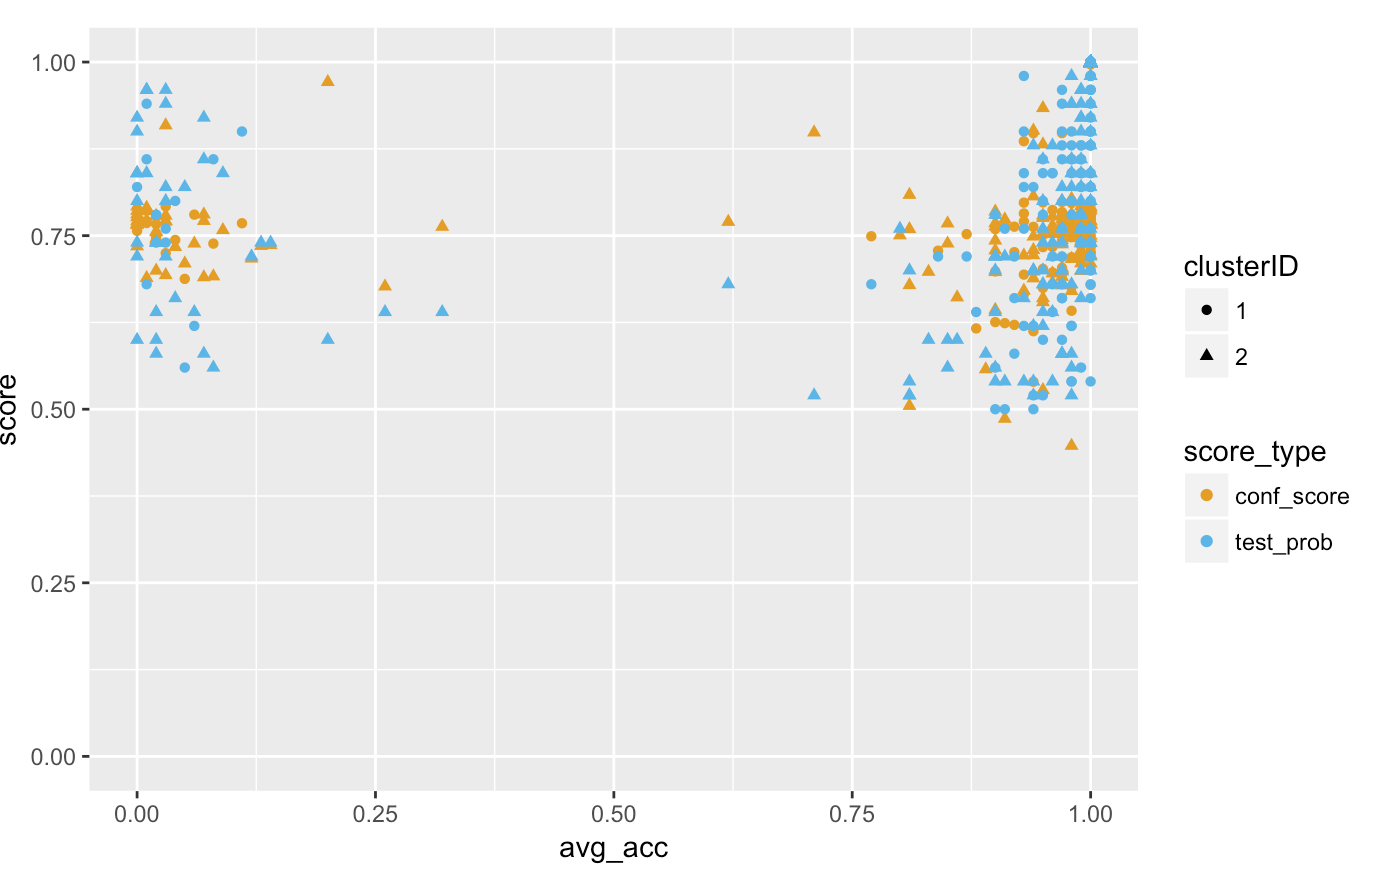
\includegraphics[width=\textwidth,height = 0.8\textwidth]{example3_1_1.png} &   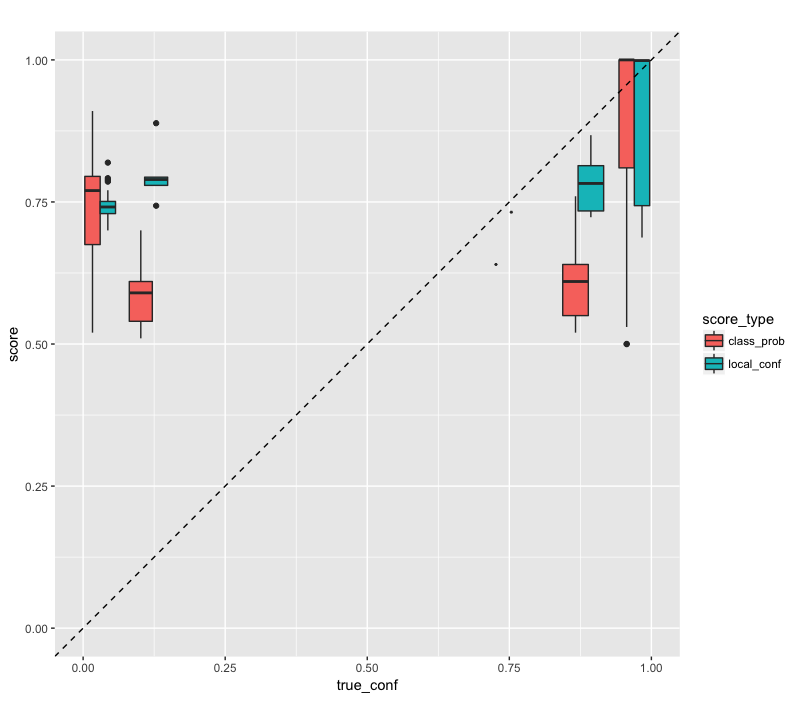
\includegraphics[width=1.1\textwidth,height = 0.8\textwidth]{example3_1_2.png} 
% \end{tabular}
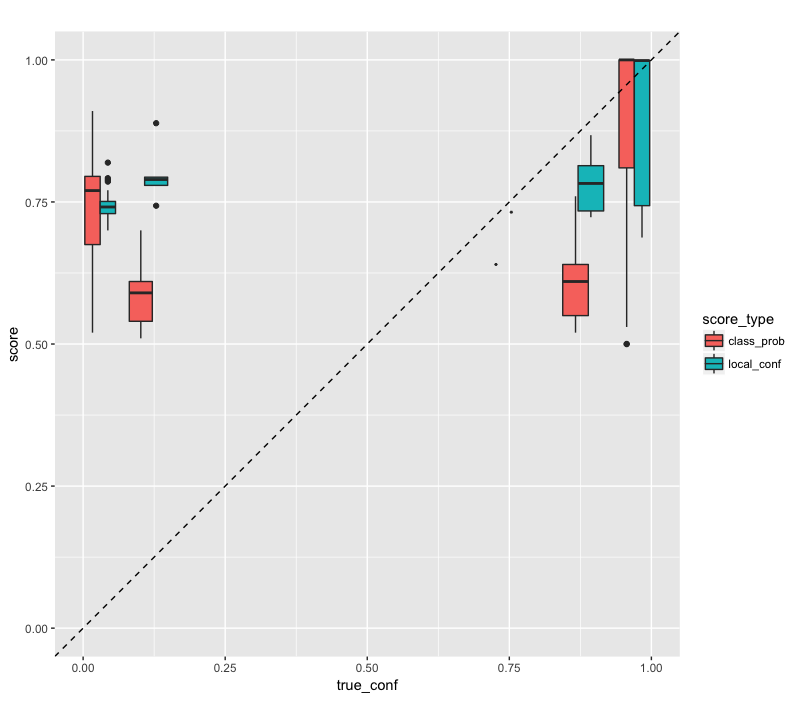
\includegraphics[width=\textwidth,height = 0.8\textwidth]{example3_1_2.png}
}
\label{fig3}
\caption{Comparisons between local confidence score and class probability on Example \ref{example3} with noisy features. All test observations are plotted.}
\end{figure}

We observe from Figure 6.5 that the relationship between class probability and local confidence score is not substantially affected by noisy features.

\vspace{3mm}

\begin{example}
\label{example4}
We next proceed with 30 informative features and 20 correlated features.

simulation($N=10,000$, $n=1000$, $m=500$, n$\_$clusters$\_$per$\_$class $= 1$, and n$\_$features$=50$, n$\_$informative$=30$, n$\_$redundant$=20$, p$\_$yellow$=0.5$, p$\_$blue$=0$.
\end{example}

\begin{figure}[h]
\centering
\label{fig4}
\resizebox{.9\textwidth}{!}{
% \begin{tabular}{cc}
%   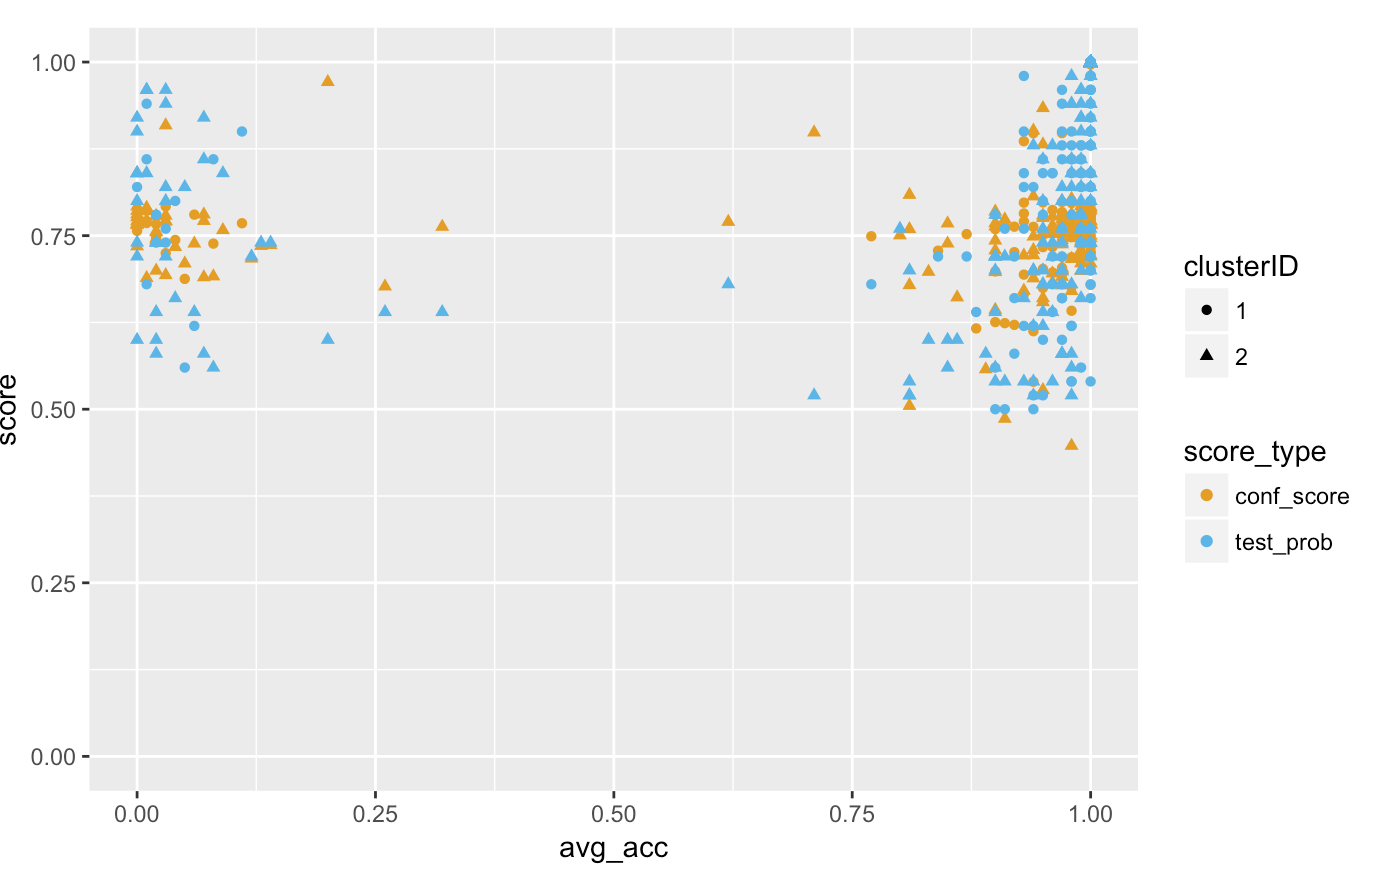
\includegraphics[width=\textwidth,height = 0.8\textwidth]{example3_1_1.png} &   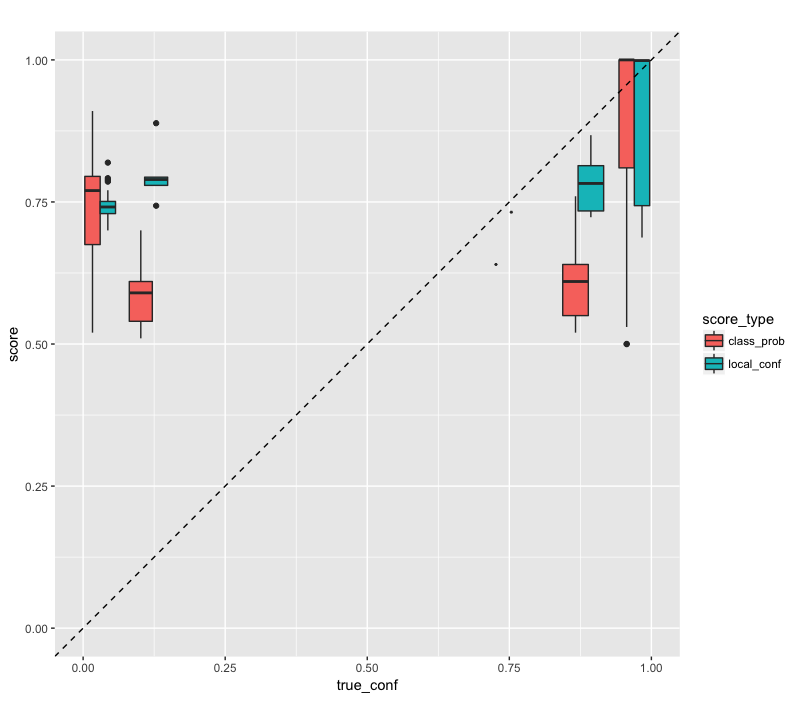
\includegraphics[width=1.1\textwidth,height = 0.8\textwidth]{example3_1_2.png} 
% \end{tabular}
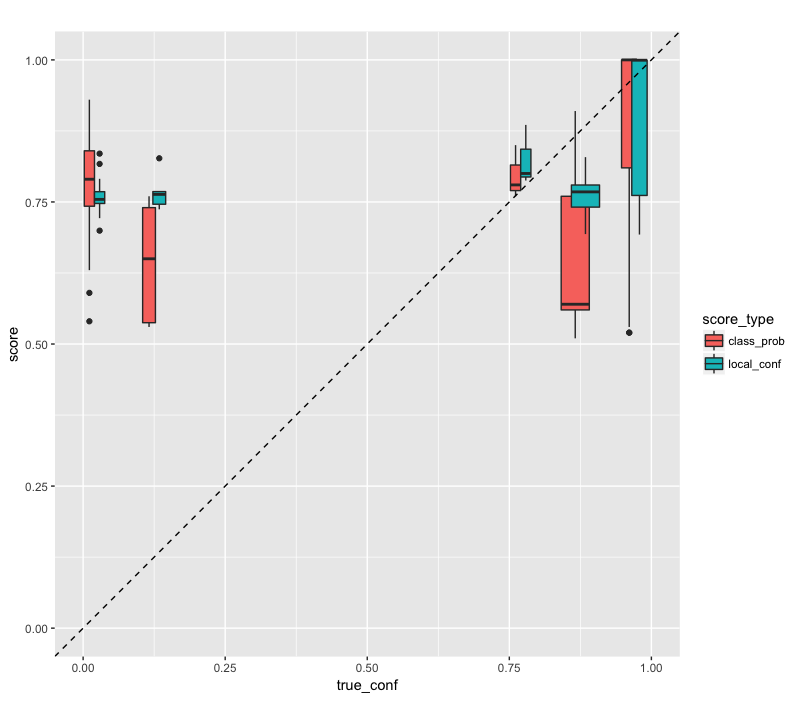
\includegraphics[width=\textwidth,height = 0.8\textwidth]{example3_2_2.png}
}

\caption{Comparisons between local confidence score and class probability on Example \ref{example4} with correlated features. All test observations are plotted.}
\end{figure}

Figure 6.6 shows that the class probability metric suffers from great variance with the presence of correlated features. In general, local confidence metric has much less variability than class probability. We can infer that this is because cohabitants are mutual: test observations that share a similar group of cohabitants mostly have very similar local confidence score. Small variance is another great property of local confidence score.

With high-dimensional data, local confidence score outperforms class probability when the true confidence is either greater than $0.5$ or smaller than $0.1$.


% \begin{figure}[h]
% \centering
% \resizebox{.9\textwidth}{!}{\begin{tabular}{cc}
%   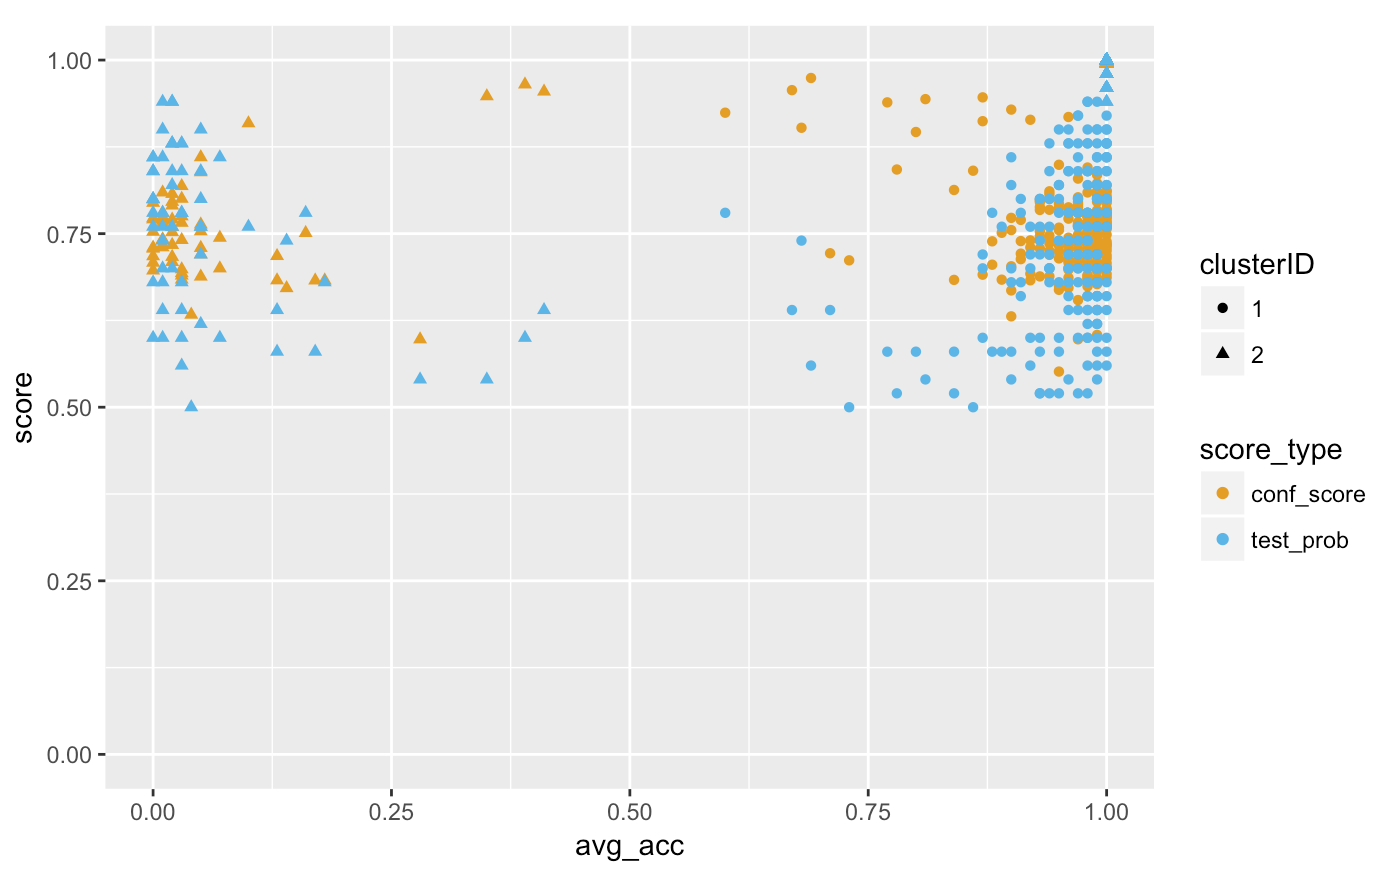
\includegraphics[width=\textwidth,height = 0.8\textwidth]{example3_2_1.png} &   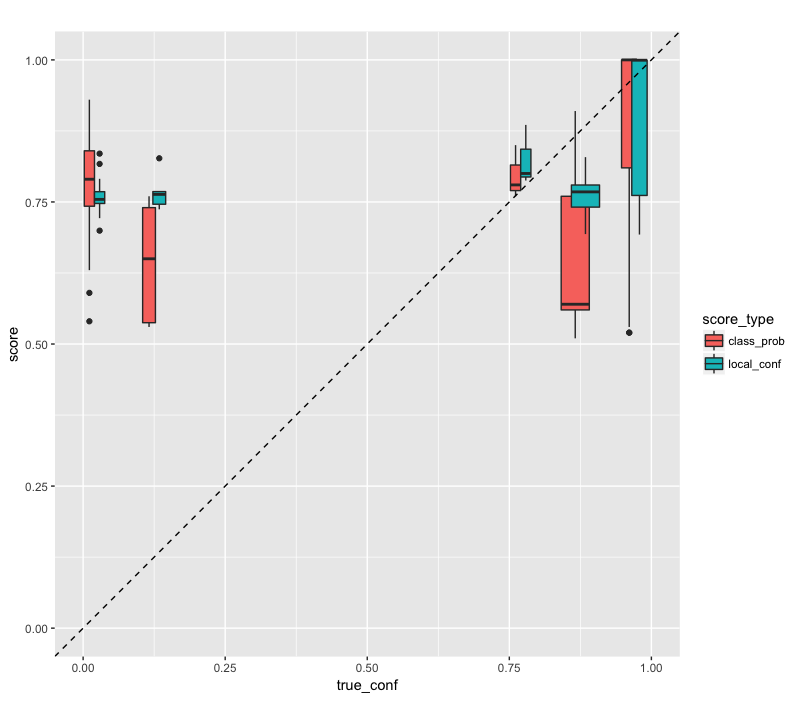
\includegraphics[width=1.1\textwidth,height = 0.8\textwidth]{example3_2_2.png} 
% \end{tabular}}
% \label{scores-example-3.2}
% \caption{Comparisons between local confidence score and class probability on Example \ref{example3.1} with correlated features. All test observations are plotted.}
% \end{figure}

% \begin{figure}[h]
% \centering
% \resizebox{1\textwidth}{!}{\begin{tabular}{cc}
%   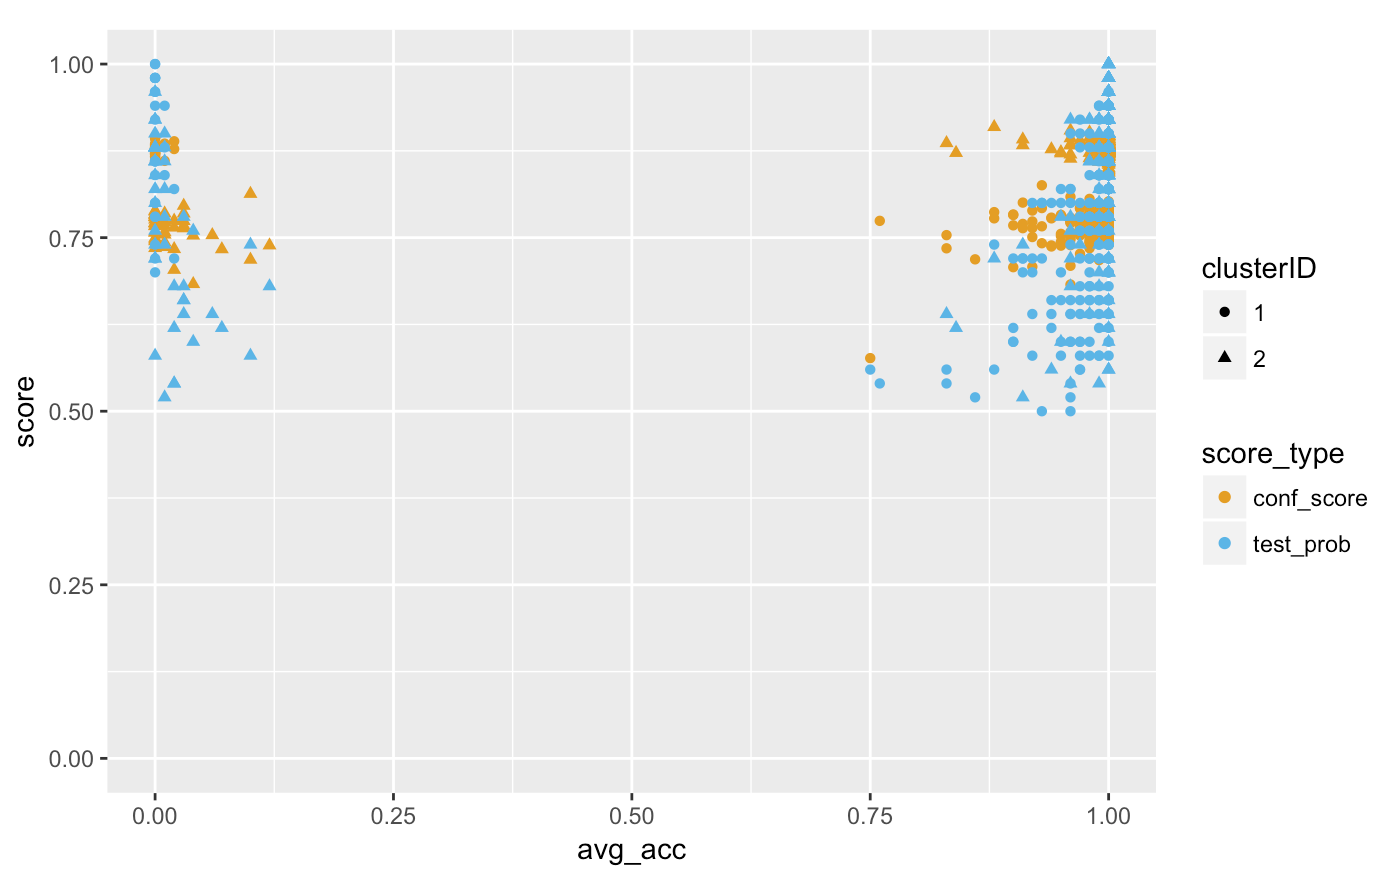
\includegraphics[width=\textwidth,height = 0.8\textwidth]{example4_1.png} &   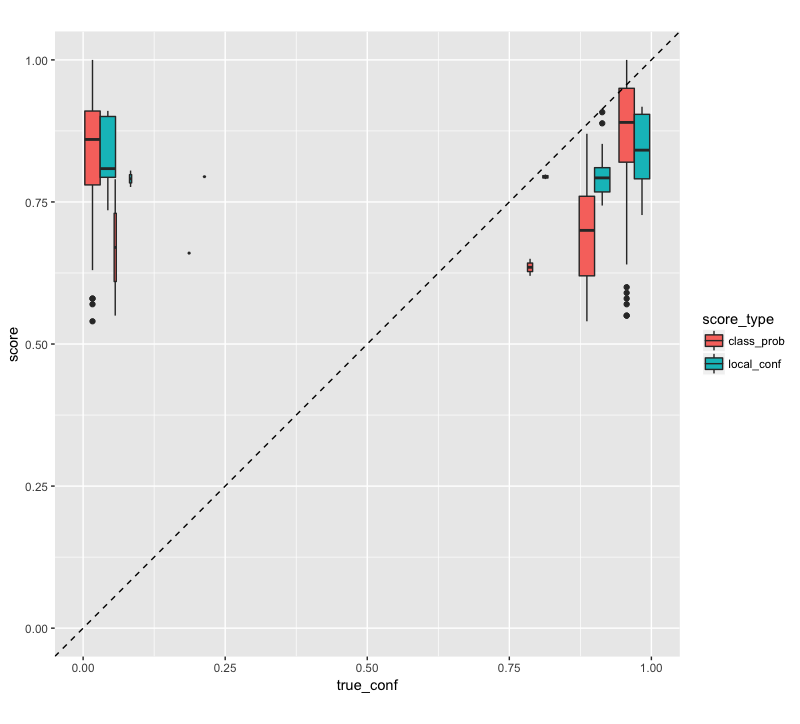
\includegraphics[width=1.1\textwidth,height = 0.8\textwidth]{example4_2.png} 
% \end{tabular}}
% \label{scores-example-4}
% \caption{Comparisons between local confidence score and class probability on Example \ref{example4} with different level of homogeneity.}
% \end{figure}

\newpage

\begin{example}
\label{example5}
After exploring dimensionality, we will take another step to simulate more interesting data with different levels of heterogeneity in the feature space. Use total number of 50 features, with 20 informative, 20 noise and 10 correlated. Simulate two clusters per class and the clusters have 50\% and 20 \% homogeneity respectively.

simulation($N=10,000$, $n=1000$, $m=500$, n$\_$clusters$\_$per$\_$class $= 1$, and n$\_$features$=50$, n$\_$informative$=20$, n$\_$repeated$=20$, n$\_$redundant$=10$, p$\_$yellow$=0.5$, p$\_$blue$=0.2$.
\end{example}


\begin{figure}[h]
\centering
\label{fig5}
\resizebox{.9\textwidth}{!}{
% \begin{tabular}{cc}
%   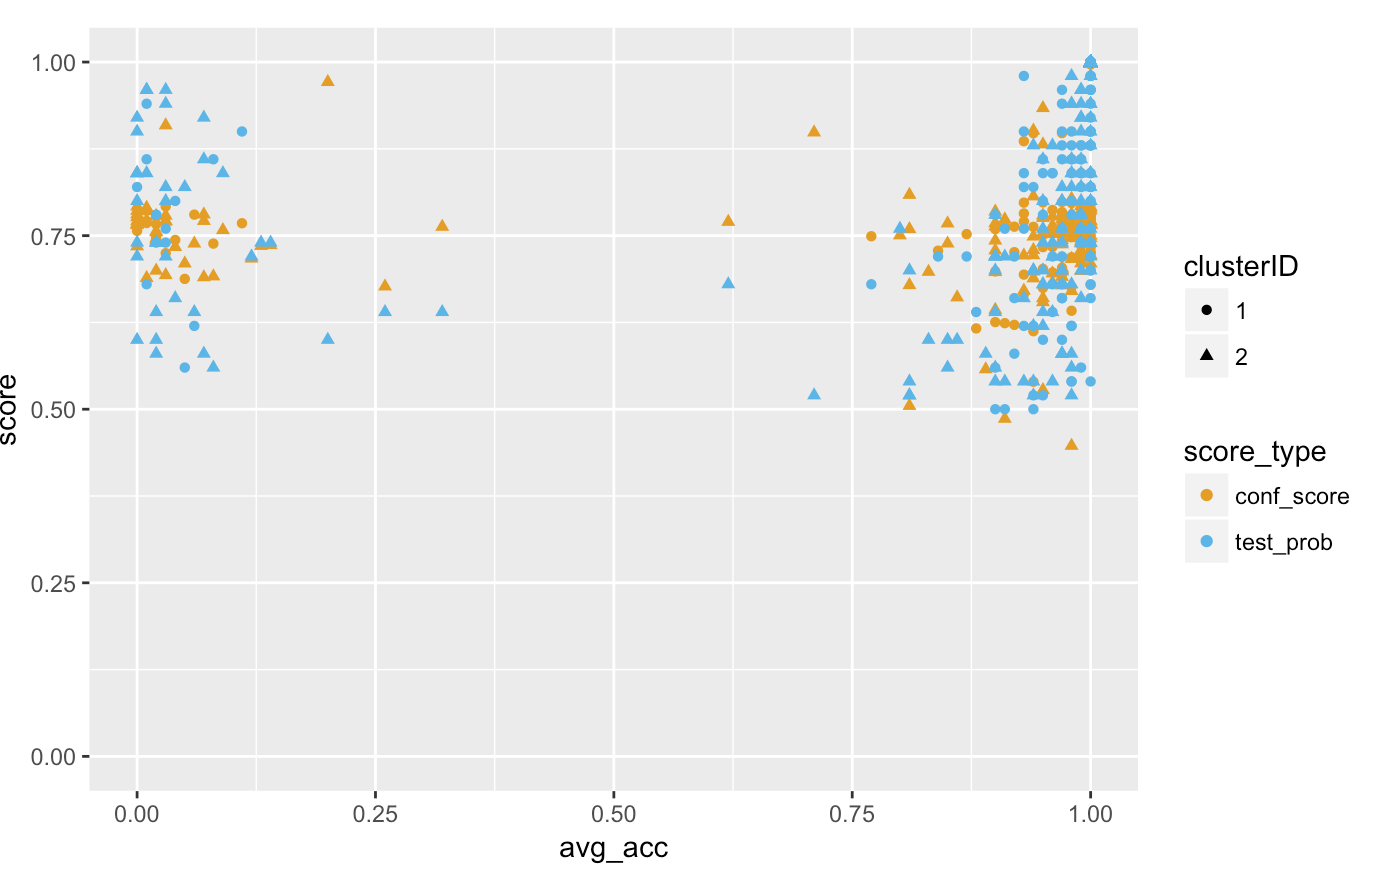
\includegraphics[width=\textwidth,height = 0.8\textwidth]{example3_1_1.png} &   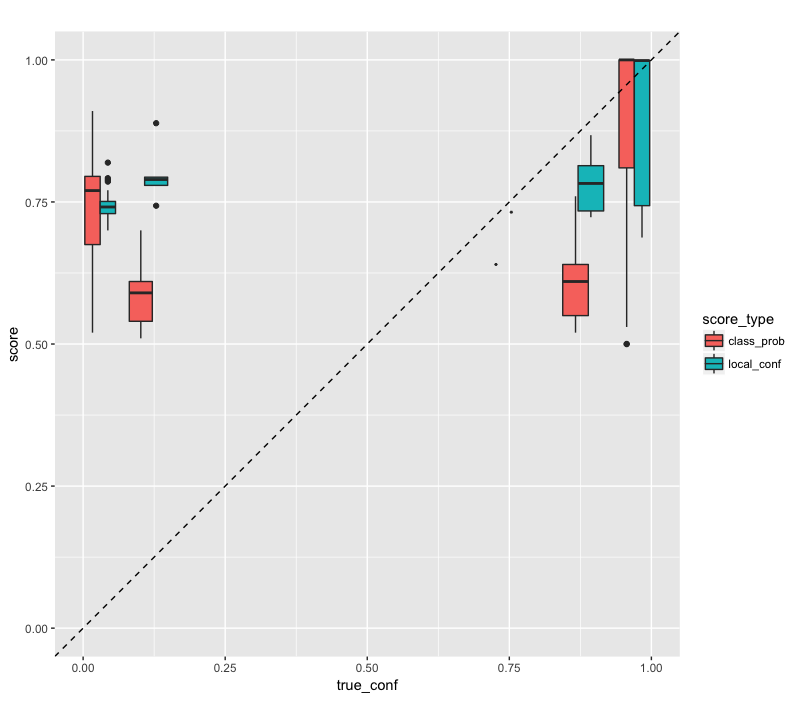
\includegraphics[width=1.1\textwidth,height = 0.8\textwidth]{example3_1_2.png} 
% \end{tabular}
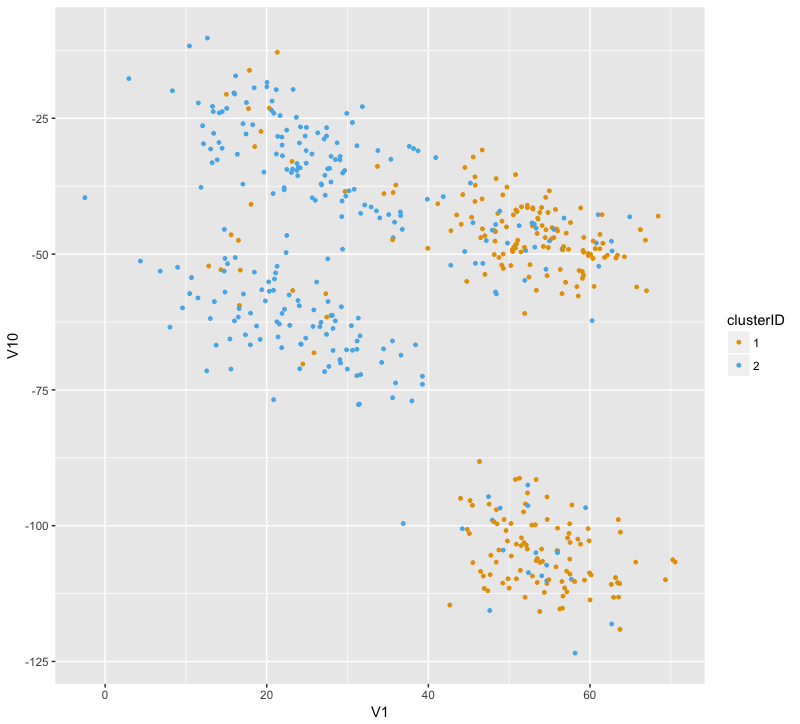
\includegraphics[width=\textwidth,height = 0.8\textwidth]{example5.png}
}
\caption{Visualization the population in Example \ref{example5}}
\end{figure}


\begin{figure}[h]
\centering
\resizebox{.9\textwidth}{!}{ 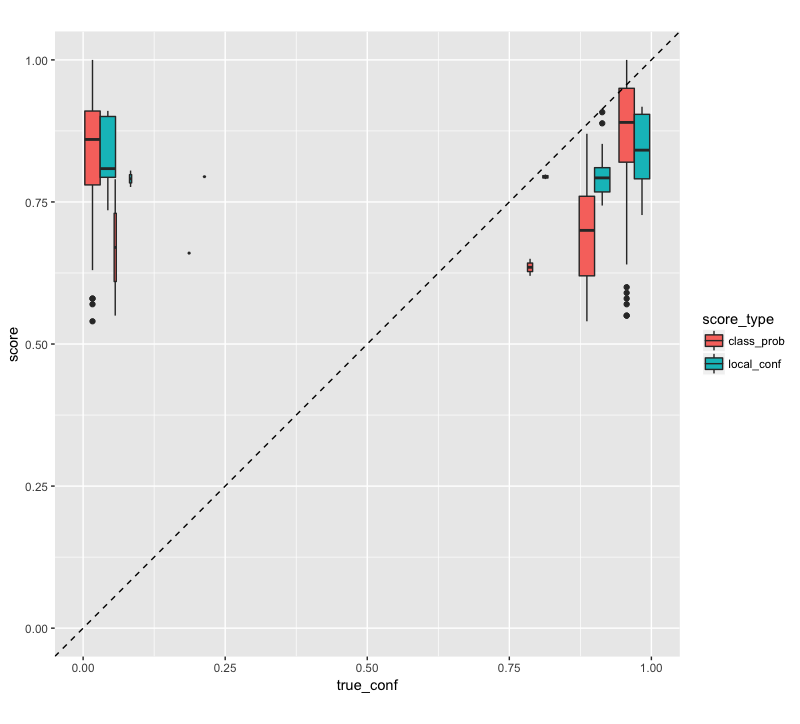
\includegraphics[width=1\textwidth,height = 0.8\textwidth]{example4_2.png} }
\label{fig6}
\caption{Comparisons between local confidence score and class probability on Example \ref{example5} with different level of heterogeneity.}
\end{figure}

Figure 6.8 shows that in this data scenario local confidence score is a closer approximation of individual prediction confidence than class probability, especially for observations with less than $100\%$ true confidence. We can also see that local confidence is conservative for observations with very high true confidence, in other words, observations in very homogeneous feature space. This can be explained by our definition of local confidence: a new observation has a local confidence of $100\%$ if and only if all its oob-cohabitants are predicted correctly by the model, which is an impossible criteria to meet since we don't perfectly fit the training data.  

In the next section, we will strengthen the claim that local confidence is a better estimator of individual prediction confidence by quantifying the differences between the confidence metrics and running comparisons on numerous simulated data. 

\section{Root Mean Square Error}

To quantify how well the confidence metrics estimate confidence, we use root mean squared error:

\begin{equation*}
   \sqrt{ \frac{1}{n}\sum_i^n(p_i-\hat{p}_i)^2}
\end{equation*}
where $n$ is the number of test observations, $p$ is the approximated true confidence, and $\hat{p}$ is either local confidence score or class probability.

Using this error metric, we will compare all the previous examples.

\begin{table}[h]
\begin{tabular}{|l|l|l|l|l|l|}
\hline
                    & example1 & example2 & example3 & example4 & example5 \\
                    \hline
local$\_$confidence    & \textbf{0.250}   & \textbf{0.304}   & \textbf{0.293}   & \textbf{0.284}    & \textbf{0.351}   \\
$p_h$    & 0.265   & 0.306   & 0.294     & 0.291     & 0.355   \\
$Acc_{oob}$ & 0.291   & 0.326   & 0.317     & 0.306     & 0.352  \\
\hline
\end{tabular}
\label{error-table}
\caption{The root mean square error between the confidence metrics and approximated true confidence for the examples in the previous section.}
\end{table}

From the table, we can conclude that for our simulations, out-of-bag accuracy is the worst method to estimate individual prediction confidence compared with local confidence and class probability. Local confidence has smaller root mean square error than class probability in all examples, but the margin is not substantial. We believe that local confidence is a very promising estimator, but we need more empirical simulations to fully support the claim.


\section{Theoretical Justification}
In addition to empirical evaluation, we also seek a theoretic grounding for our proposed local confidence using a probabilistic estimation framework. The probability calibration in this section is based on \cite{Olson}. 

Prediction confidence can be interpreted as the probability that the model predicts the response correctly given its feature space. 
To put it formally, let $z_1,...z_n$ be the set of training observations, and $z_i = (x_{i_1},...x_{i_p})$ $\forall i \in 1,...n.$. Let $y_1,...y_n$ be the categorical response variable. Let $z_h$ be a new observation and $x_h$ be its feature space. Then we can define the prediction confidence of $z_h$ as 
$$P(\hat{y}_h=y_h|x_h)$$

Using Bayes' Rule, we can further write this probability as 
\begin{equation} \label{eq1}
\begin{split}
P(\hat{y}_h=y_h|x_h) &= \frac{P(\hat{y}_h=y_h)P(x_h|\hat{y}_h=y_h)}{P(x_h)} \\
  & \approx \frac{\hat{P}(\hat{y}_h=y_h)\hat{P}(x_h|\hat{y}_h=y_h)}{\hat{P}(x_h)}
\end{split}
\end{equation}

We can interpret the cohabitance frequency as a proximity function, that is $w(z_h,z_i)$, the number of times a training observation $z_i$ out-of-bag cohabs with $z_h$, is large if $z_i$ and $z_h$ are similar to each other and small vice versa. Then 
\begin{equation}
    \hat{P}(x_h) \equiv \frac{1}{n} \sum_{i=1}^n  w(z_i,z_h)
\end{equation}
Furthermore
\begin{equation}
  \hat{P}(x_h|\hat{y}_h=y_h) \equiv \frac{1}{n_1}\sum_{i=1}^n w(z_h,z_i)\mathbb{I}(\hat{y}_i=y_i) 
\end{equation}
where $n_1$ is the number of oob training samples that are predicted correctly. 
Let 
\begin{equation}
   \hat{P}(\hat{y}_h=y_h) = \frac{n1}{n} = Acc_{oob} 
\end{equation}
the oob prediction accuracy. Then 
\begin{equation} \label{eq2}
\begin{split}
P(\hat{y}_h=y_h|x_h) 
  & \approx \frac{\hat{P}(\hat{y}_h=y_h)\hat{P}(x_h|\hat{y}_h=y_h)}{\hat{P}(x_h)} \\
  & = \frac{\sum_{i=1}^n w(z_h,z_i)\mathbb{I}(\hat{y}_i=y_i) }{ \sum_{i=1}^n  w(z_i,z_h)} \\
  & = local\_confidence
\end{split}
\end{equation}

Together with empirical evaluation, we made a convincing case that our proposed local confidence improves current estimation of individual prediction confidence. 
\end{chapter}

%%%%%%%%%%%%%%%%%%%%%%%%%%%%%%% DISCUSSION ON OTHER MODELS %%%%%%%%%%%%%%%%%%%%%%%%%%%%
\begin{chapter}{Applications and Future Directions}
After empirically and theoretically evaluating our proposed local confidence and the other currently existing confidence metrics, the next pressing question to ask is, to whom is our proposed method useful? What are limitations of the local confidence score in wider applications?

Recall that local confidence represents the prediction confidence of an individual new observations, and that it better captures the heterogeneity in the feature space. Our result will be helpful to researchers whose work emphasizes individual predictions. Estimating individual outcome probabilities has applications in medicine, particularly diagnosis, decision on therapy or prognosis \citep{Dankowski}. 

Local confidence does fall short when we have minorities sharing feature space with observations from predominately the opposite class. If the cohabitants are from the other class and are predicted almost perfectly, the minority will always be predicted as the majority and local confidence score will never reflect the true prediction accuracy. However, no other known methods can overcome such shortcoming.  

Since the scope of the empirical evaluation in this thesis focuses only on binary classification, looking into the future, more simulations can be done in multiclass classification. In addition, our proposed local confidence can be further tested on real-world data, such as the \href{https://archive.ics.uci.edu/ml/datasets.php}{UCI Machine Learning Datasets}, to obtain a universal benchmark for comparisons of confidence metrics in other literature and ours.

The random forests we trained are the very first one created by \cite{Breiman}. Yet we should not forget that there have been substantial research advancements in optimizing random forests in recent years. In \cite{WagerJMLR}, a local estimation is proposed to assign more weights to training samples that are similar to the test observations when building the forests. It would be very interesting to see the performance of the local confidence metrics on random forests that are further optimized. 


\end{chapter}

\begin{chapter}{Conclusion}
Despite many literature in prediction intervals in regression, prediction confidence in classification random forests are predominately global metrics. Although class probability provides a probability estimation, very little is discussed on how that probability is related to the true prediction confidence. In this paper, we define local prediction confidence in a similar fashion as frequentist confidence intervals, as the prediction accuracy of one observation over repeated training samples. 

We developed local prediction confidence directly using the random forests structure. The local prediction confidence of a new observation is approximated by the prediction accuracy of out-of-bag training observations that frequently oob-cohab with the new observation. We then simulated data sets of different dimensionality and homogeneity and evaluated local confidence along with class probability and out-of-bag accuracy. 

We have empirically shown that local confidence better captures the heterogeneity of the feature space than other global metrics. We also observe that local confidence score gives a more accurate estimate of the true prediction confidence than class probability, and the estimator itself has smaller variance. In addition to empirical evaluation, we also showed theoretic justification using probability estimation.

The results offer a promising first step, yet additional work remains to be done. More simulations can be conducted to provide more concrete evidence, and real data set can be used to further test the differences of the metrics. 
\end{chapter}


\begin{chapter}{Appendix}
The R script that calculates local confidence is attached. 

\begin{verbatim}
    #####
# A function that calculates the local prediction confidence of a test dataset
# parameters: 
# inbag_counts: the number of times each training observation is  
in bag in all trees
# trainNodes: train nodes returned by ranger
# testNodes: the test nodes returned by ranger
# train_response: the response of the training observations
# train_pred: training predictions
# test_response: the response of test observations
# test_pred: test predictions


library(ranger)

# return a frequest list of all training observations 
# each element stores the number of times each training observation 
is oob-cohab with x
getFreq<- function(inbag_counts,trainNodes,testNodes,x){
  freq_lst<-rep(0,nrow(trainNodes))
  for (b in 1:ncol(trainNodes)){
    node_x<-testNodes[x,b] # the terminal node ID of x
    oob_cohab<-which(trainNodes[,b]==node_x & inbag_counts[[b]]==0)
    freq_lst[oob_cohab]=freq_lst[oob_cohab]+1
  }
  return(freq_lst)
}

# get the cohabitant of test observation x
getCohabitant <- function(inbag_counts,trainNodes,testNodes,x){
  freq_lst <- getFreq(inbag_counts,trainNodes,testNodes,x)
  return(which(freq_lst>0))
}

# return a list of lists of each test observation's cohabitant.
getAllCohabitant <- function(inbag_counts,trainNodes,testNodes){
  all_cohabs <- list()
  for (i in 1:nrow(testNodes)){
    cohabs <- getCohabitant(inbag_counts,trainNodes,testNodes,i)
    all_cohabs[[i]]<-cohabs
  }
  return(all_cohabs)
}

# return the confidence score of x
confidence<-function(inbag_counts,trainNodes,testNodes,
train_pred,train_response,x){
  accuracy<-allAccuracy(inbag_counts,train_pred,train_response)
  weight<-getFreq(inbag_counts,trainNodes,testNodes,x)
  score<-sum(accuracy*weight)/sum(weight)
  return(score)
}

#  return the confidence score of all test responses
allConfidence<-function(inbag_counts,trainNodes,testNodes,
train_pred,train_response){
  lst<-rep(0,nrow(testNodes))
  for (x in 1:nrow(testNodes)){
    conf<-confidence(inbag_counts,trainNodes,testNodes,train_pred,
    train_response,x)
    lst[x] = conf
  }
  return(lst)
}


## get out of bag prediction accuracy for training sample m
oobAccuracy <- function(m,inbag_counts,train_pred,train_response){
  oob_pred <- rep(0,ncol(train_pred))
  for(b in 1:ncol(train_pred)){
    if(inbag_counts[[b]][m]==0){
      oob_pred[b] <- train_pred[m,b]
    }
  }
  
  oob_pred <- oob_pred[oob_pred>0]
  
  final_pred <-as.numeric(names(which.max(table(oob_pred))))
  return(final_pred==train_response[m])
}

# get out of bag training accuracy for all training observations
allAccuracy<-function(inbag_counts,train_pred,train_response){
  allAcc<-rep(0,nrow(train_pred))
  for (m in 1:nrow(train_pred)){
    acc<-oobAccuracy(m,inbag_counts,train_pred,train_response)
    allAcc[m]=acc
  }
  return(allAcc)
}


\end{verbatim}
\end{chapter}

% the bibliography
% {99} basically says that you need to leave two spaces for each item number
\bibliographystyle{apalike}
\bibliography{reference.bib}

\end{document}



